% Euclidean Geometry Solutions
% Started in Summer 2020
\documentclass{tufte-handout}

%\geometry{showframe}% for debugging purposes -- displays the margins

%%%% Packages to make things pretty
\usepackage{amsmath,amsthm}
\usepackage{booktabs}
\usepackage{graphicx}
\setkeys{Gin}{width=\linewidth,totalheight=\textheight,keepaspectratio}
\graphicspath{{graphics/}}
\usepackage{units}
\usepackage{fancyvrb}
\fvset{fontsize=\normalsize}
\usepackage{multicol}
\usepackage{pdfpages}

%%%% Theorem Environments
\theoremstyle{definition}
\swapnumbers
\newtheorem{theorem}{Theorem}[section]
\newtheorem{definition}[theorem]{Definition}
\newtheorem{lemma}[theorem]{Lemma}
\newtheorem{corollary}[theorem]{Corollary}
\newtheorem{postulate}[theorem]{Postulate}

%%%%%

\title[Solutions]{Solutions to Euclidean Geometry Tasks}
\author[Hitchman]{Theron J Hitchman}
\date{\today}

\begin{document}

\maketitle

\begin{marginfigure}
    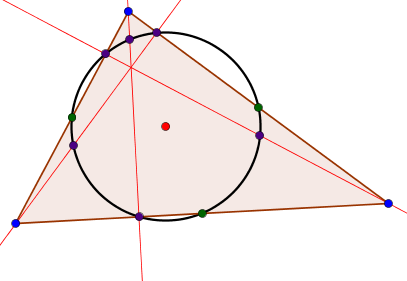
\includegraphics{images/NPC.png}
\end{marginfigure}

%%%% \setcounter{section}{-1}
\section*{Introduction}

I collect here solutions to the standard sequence of Euclidean Geometry tasks. As time goes on, I might add solutions devised by my students. For now I will just put down my favorite solution, without trying to figure out if it is one of mine, or one written by a student at some point in the last 12 years.

My thanks to all of my students, who have helped me to enjoy our time together doing mathematics by being clever, persistent, and open to learning new ways of thinking.

I'll do this section by section, but I won't necessarily do the tasks in order inside a given section. Instead, I will work through the material in a way that fits how I think about it. In particular, this means that the numbering of results here, given as [section].[item], will not necessarily match the numbering used in the notes. The section numbers will be the appropriate, but in each section the theorems might be proved in a different order. In fact, as one question or another might produce several different results as ``answers,'' the number of results generally does not match the number of questions.


\setcounter{section}{1}
\section{Beginnings: The Rhombus}\label{section:rhombi}

\begin{theorem}[Conjecture 1.1]\label{theorem:rhombus-opp-angles}
Let $ABCD$ be a rhombus. Then angle $ABC$ is congruent to angle $ADC$. Similarly, angle $BAD$ is congruent to angle $BCD$.
\end{theorem}

\begin{proof}
By Postulate 1, we may draw in the segment $AC$. This divides our rhombus into two triangles, triangle $ABC$ and triangle $ADC$.

\begin{marginfigure}
  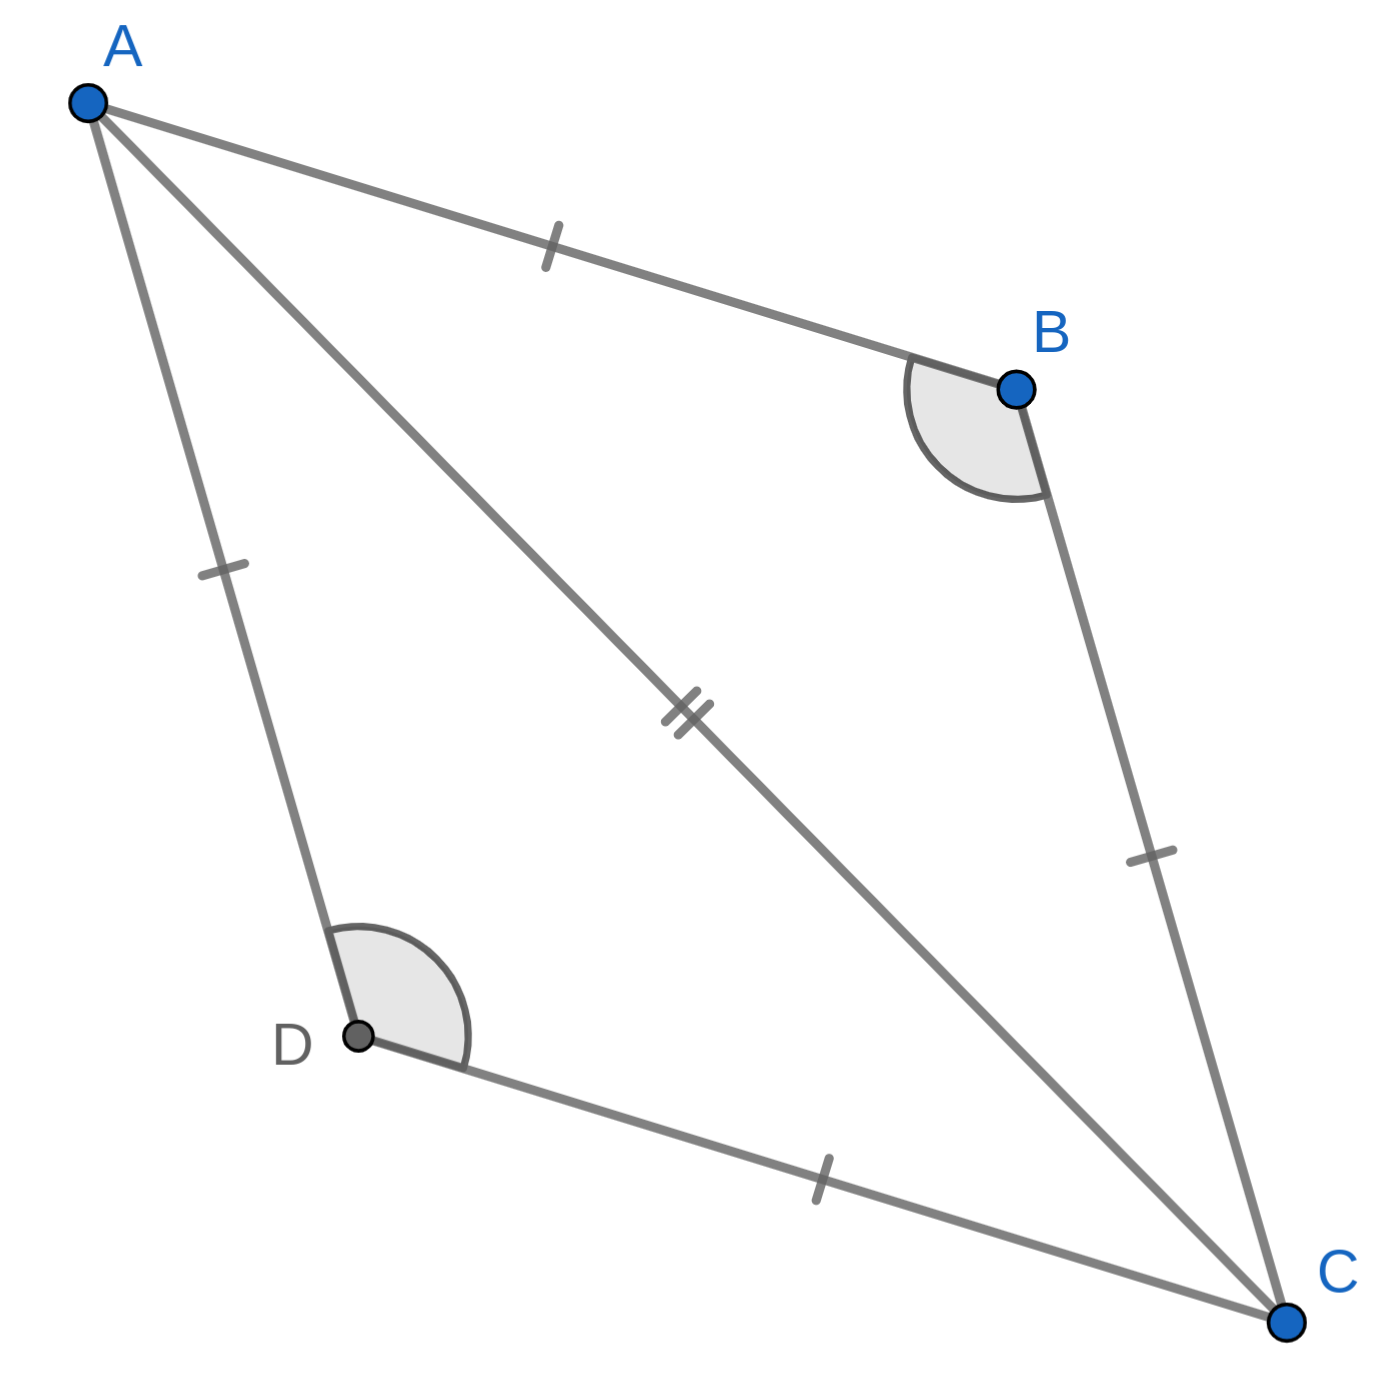
\includegraphics{images/rhombus_with_diagonal.png}
\end{marginfigure}

Since our original figure is a rhombus, we know that the four segments $AB$, $BC$, $CD$, and $DA$ are all congruent. In particular, $AB$ is congruent to $AD$ and $BC$ is congruent to $DC$. Also, the segment $AC$ is shared by both triangles and is congruent to itself. Therefore, by Euclid's proposition I.8, the two triangles $ABC$ and $ADC$ are congruent.

Since the two triangles are congruent, their corresponding angles are congruent, by the definition of congruent triangles. We conclude that angle $ABC$ is congruent to angle $ADC$.

We can obtain the second conclusion by entirely similar reasoning, but instead dividing the rhombus by the segment $BD$.
\end{proof}

\begin{corollary}\label{corollary:rhombus-angle-bisectors}
Let $ABCD$ be a rhombus. The diagonal $AC$ is an angle bisector for both angle $BAD$ and angle $BCD$.

Moreover, the diagonal $AC$ divides the rhombus into a pair of congruent isosceles triangles, with base angles sitting on the diagonal.
\end{corollary}

\begin{proof}
As in the proof of the theorem, we know that the triangles $ABC$ and $ADC$ are congruent. But since $ABCD$ is a rhombus, we also know that these triangles are isosceles. Since all four sides of the rhombus are congruent, we know that $AB$ is congruent to $BC$ and $AD$ is congruent to $DC$.

\begin{marginfigure}
  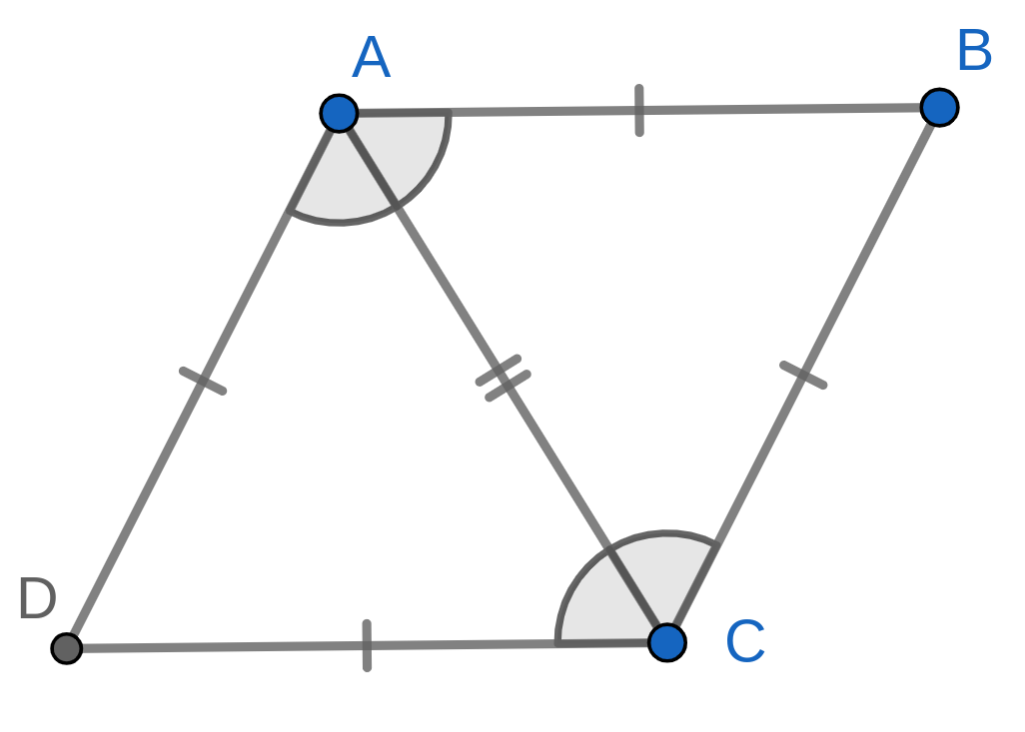
\includegraphics{images/rhombus_diagonal_marked.png}
\end{marginfigure}

So by Eulid's Proposition I.5, we conclude that the angles
$BAC$ and $BCA$ are congruent. The same holds for the angles $DAC$ and $DCA$. But these pairs of angles can be made to correspond to each other in the triangle congruence between triangle $ABC$ and triangle $ADC$. Therefore, all four of these angles must be congruent.

In particular, this means that the ray $AC$ cuts the angle $BAD$ into two congruent pieces: angle $BAC$ and angle $DAC$. Thus, $AC$ is the angle bisector of angle $BAD$. Similarly, $AC$ is the angle bisector of angle $BCD$.
\end{proof}

\begin{lemma}\label{lemma:rhombus-equilateral-triangles}
The three angles of an equilateral triangle are mutually congruent. Further, those angles are each congruent to two thirds of a right angle.
\end{lemma}

\begin{proof}
Let $ABC$ be an equilateral triangle. Since $AB$ is congruent to $AC$, by Euclid's Proposition I.5 angle $ABC$ is congruent to angle $ACB = BCA$.

Also, similarly since $BC$ is congruent to $BA$, by Proposition I.5 angle $BCA$ is congruent to angle $BAC = CAB$.

By a common notion,\sidenote{We won't quote common notions anymore after this.} all three of the angles $ABC$, $BCA$ and $CAB$ are congruent. By Euclid's Proposition I.32, these three angles taken together make two right angles. Therefore, each of these angles is congruent to two thirds of a right angle.
\end{proof}

\clearpage

\begin{theorem}[Conjecture 1.1]\label{theorem:rhombus-not-square}
There is a rhombus $ABCD$ such that angle $BAC$ and $BDC$ are not congruent.
\end{theorem}

\begin{proof}
We shall construct such a rhombus directly. The idea is to use the method of construction in Euclid's Proposition I.1.

Pick a pair of points $A$ and $C$. Use Postulate 3 to construct circles $AC$ and $CA$. By the Circle-Circle Intersection Property,\sidenote{This is an extra axiom discussed in the introductory notes given to students.} these two circles meet at two points. We call these two points $B$ and $D$. Finally, join up these points with Postulate 1 to form segments $AB$, $BC$, $CD$, and $DA$. By the argument in Euclid's Proposition I.1, this figure $ABCD$ is a rhombus.

\begin{marginfigure}
  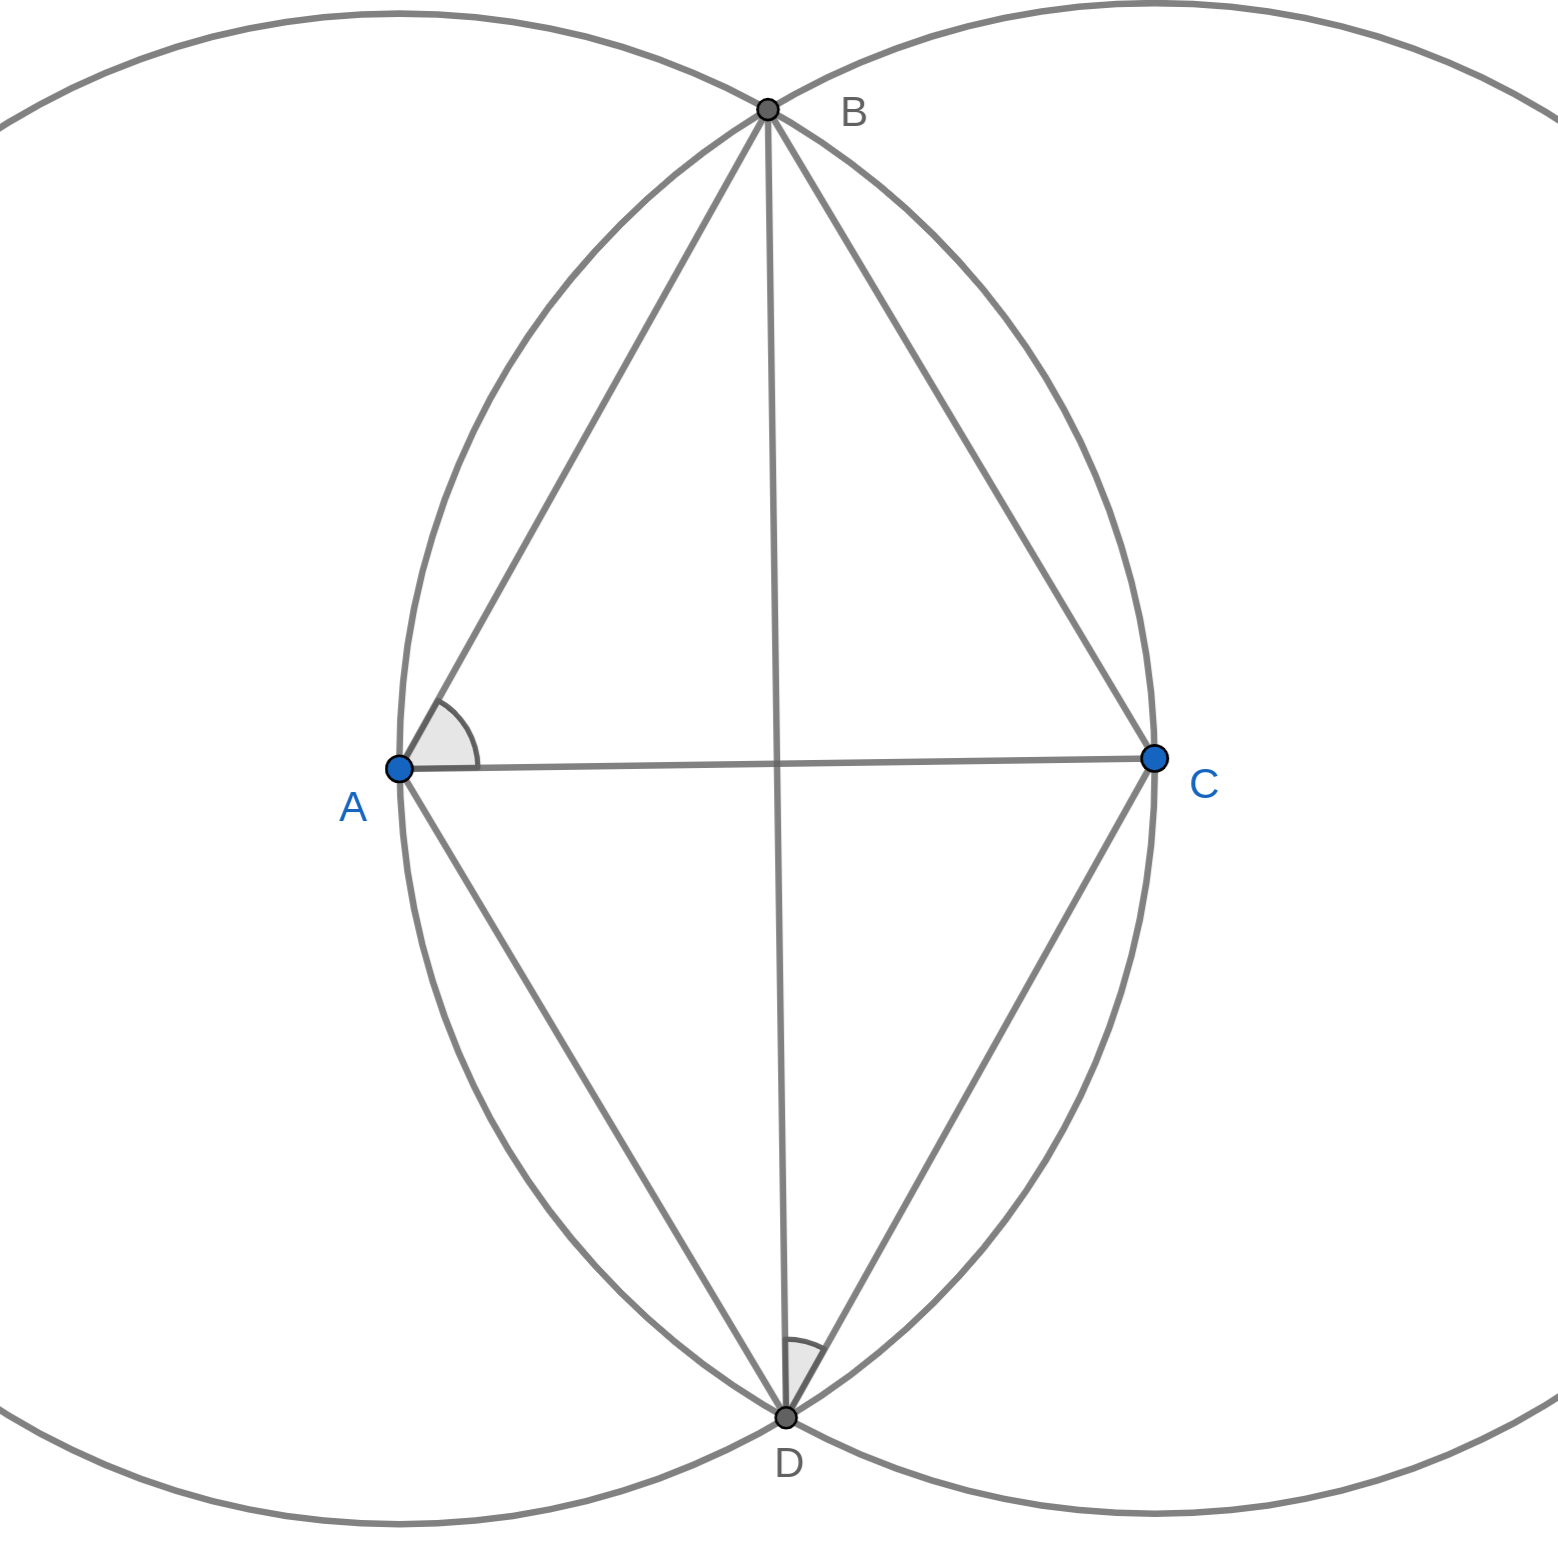
\includegraphics{images/double_equilateral.png}
\end{marginfigure}

However, we have built an interesting and special rhombus, made of two equilateral triangles with a shared side. The angle $BAC$ is one of the angles in one of these equilateral triangles.

Now draw segment $BD$ by Postulate 2. Note that angle $BDC$ is only part of angle $ADC$, so by a common notion $BDC$ is less than $ADC$. Note that angle $ADC$ is one of the angles in one of the equilateral triangles. So angle $ADC$ is congruent to angle $BAC$.

If we put these together, we see that angle $BDC$ is less than angle $BAC$. Thus these two angles are not congruent.
\end{proof}

\begin{theorem}[Conjectures 1.4 \& 1.5]\label{theorem:rhombus-construction}
Given a segment $AB$ and an angle $XYZ$, there exists a rhombus $ABCD$ with the angle at $A$ congruent to angle $XYZ$.
\end{theorem}

\begin{proof}
We will construct a rhombus directly. First, by Postulate 3 we may draw a circle $AB$, with center at $A$ and passing through $B$. By Postulates 2 and 1, in that order, draw the line through $A$ and $B$. By Euclid's Proposition I.23 we construct a ray $r$ with initial point $A$ so that this ray makes an angle with line $AB$ congruent to angle $XYZ$. Where $r$ meets the circle $AB$, mark the point $D$.

\begin{marginfigure}
  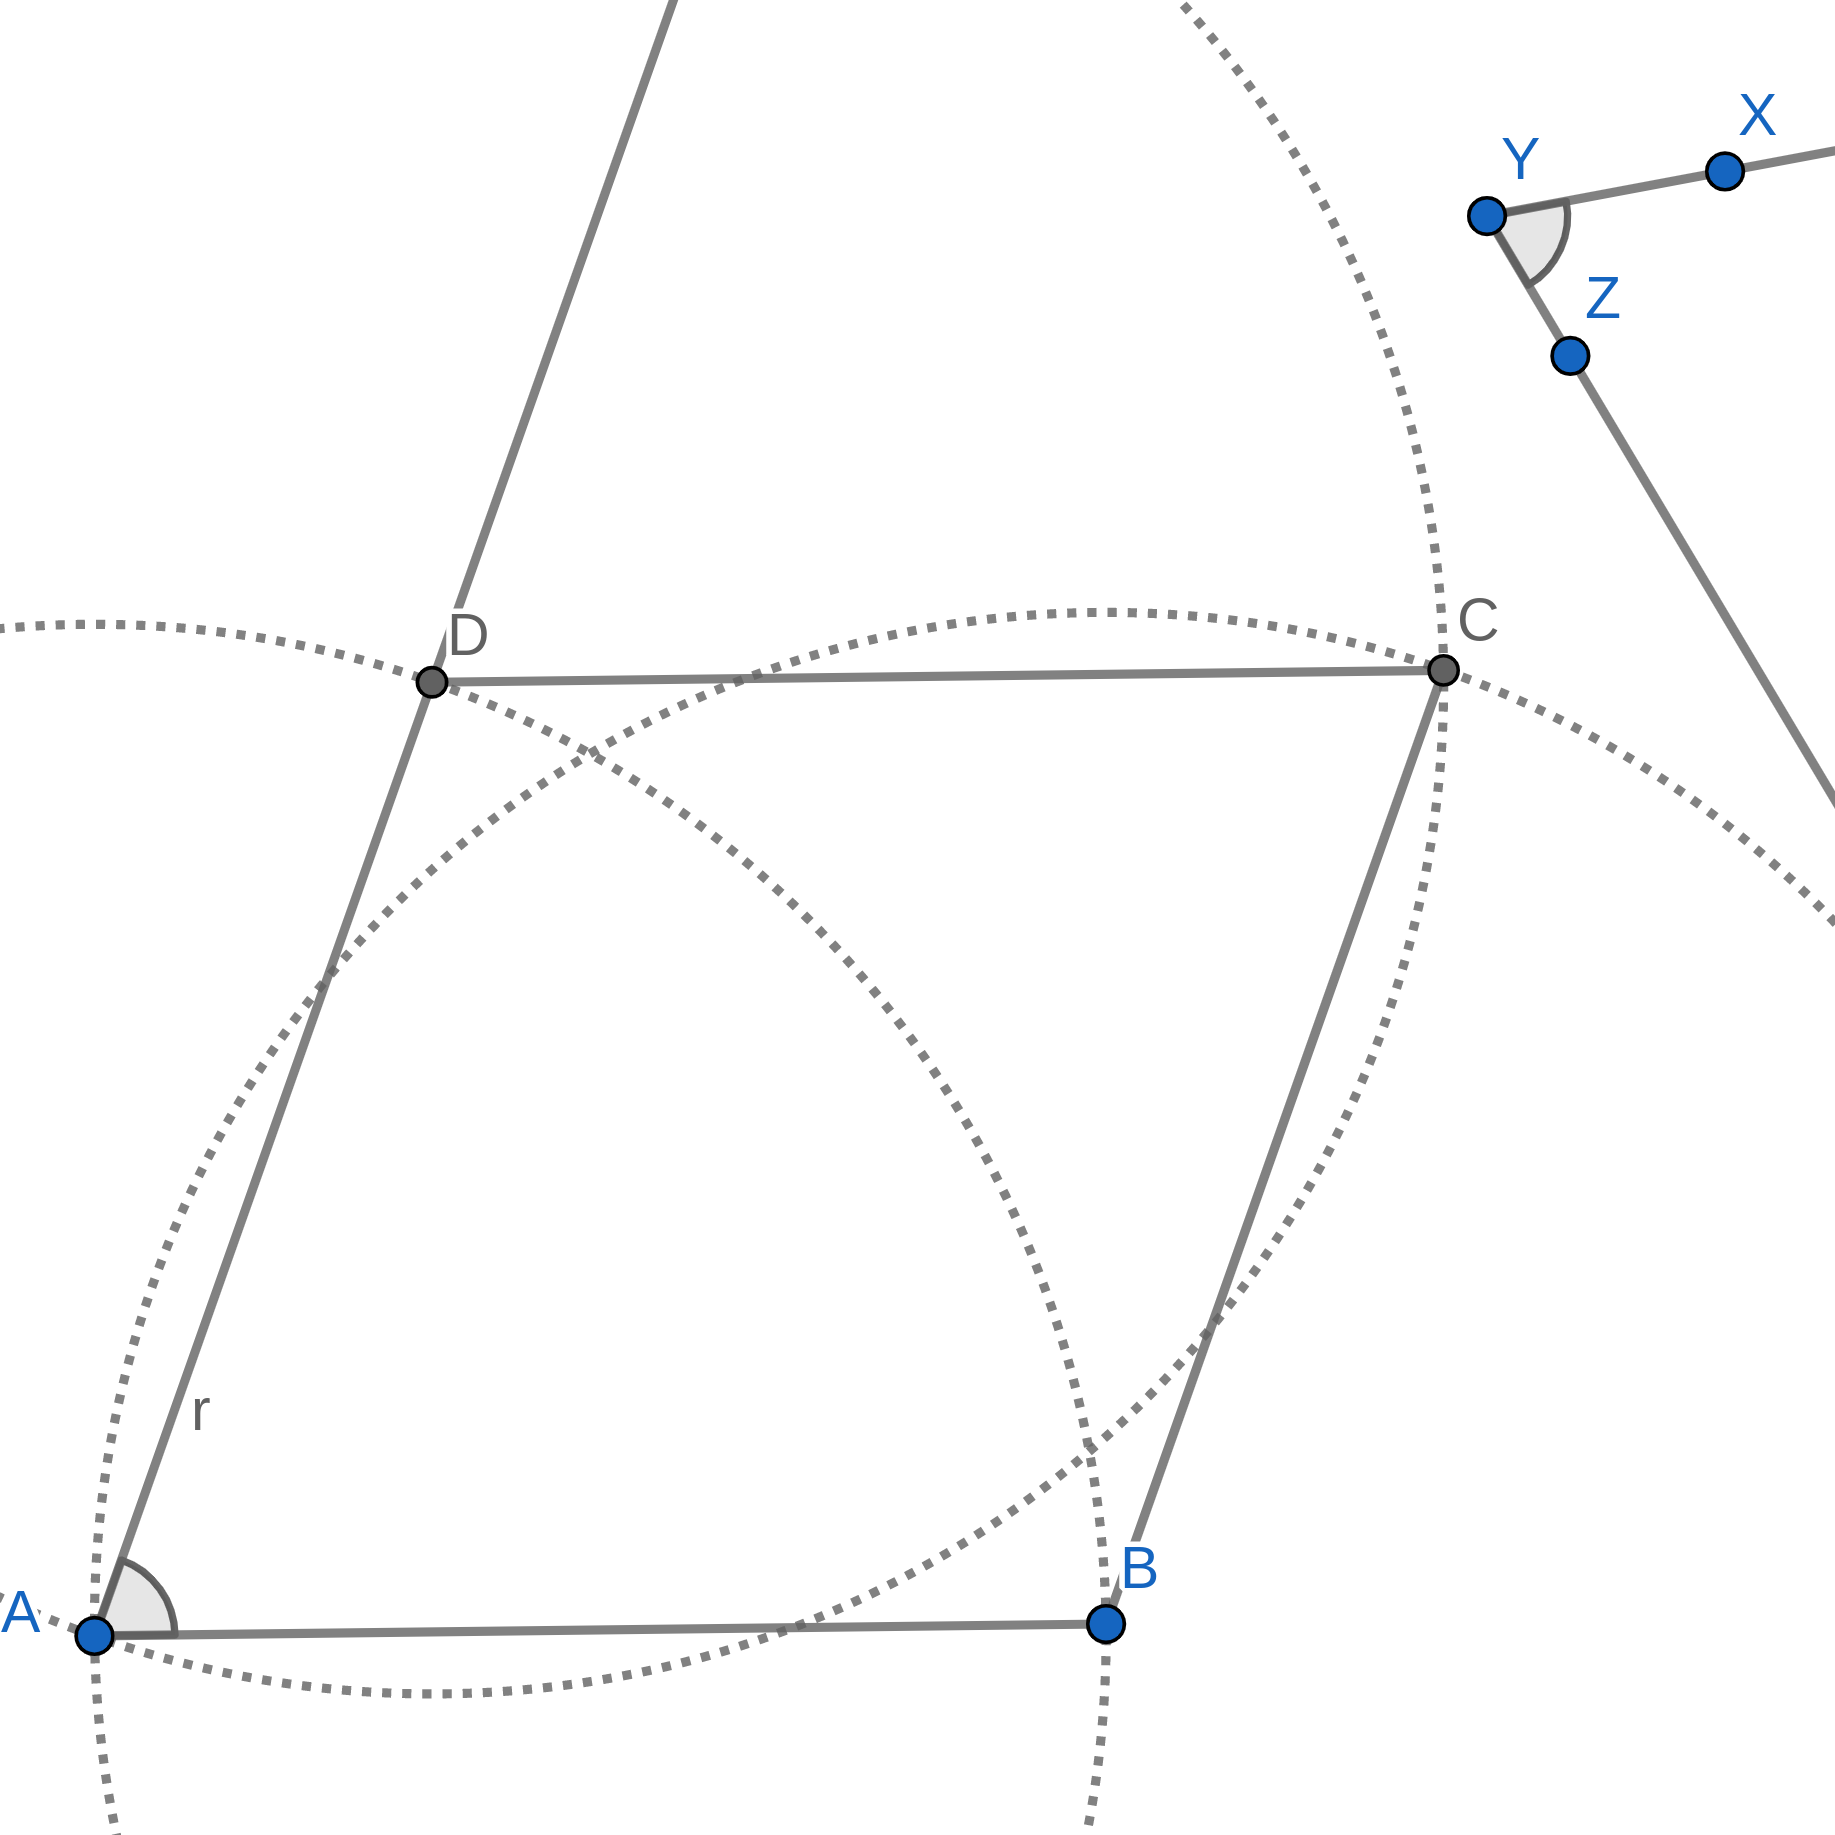
\includegraphics{images/rhombus_construction.png}
\end{marginfigure}


Now draw two more circles: circle $DA$ with center $D$ and passing through $A$ and circle $BA$ with center $B$ also passing through $A$. These two circles meet at $A$. By the Circle-Circle Intersection Property, they also meet at another point, which we call $C$.

Finally we draw the remaining required line segments to make the rhombus. By Postulate 2, we draw $BC$ and $CD$. We claim that the resulting quadrilateral $ABCD$ is the one required.

By construction, the angle $DAB$ is congruent to angle $XYZ$. Segments $AB$ and $AD$ are radii of the common circle $AB$, so they are congruent by the definition of a circle. Similar reasoning shows that $AD$ is congruent to $DC$, and $DC$ is congruent to $BC$. Therefore, all four sides of $ABCD$ are mutually congruent, and hence $ABCD$ is a rhombus.

\end{proof}



\begin{definition}[Parallelogram, inferred from Euclid I.33] \label{definition:parallelogram}
A quadrilateral $ABCD$ is a \emph{parallelogram} if for each pair of opposite segments, extending those segments to lines makes a pair of parallel lines.
\end{definition}


\begin{theorem}{Conjecture 1.6}\label{theorem:rhombus-parallelogram}
Suppose that $ABCD$ is a rhombus. Then $ABCD$ is a parallelogram.
\end{theorem}

\begin{proof}
Consider the rhombus $ABCD$, and extend the four sides to lines using Postulate 2. Also, by Postulates 1 and 2, draw the line $AC$ containing the diagonal segment $AC$. We will show that the lines $AB$ and $CD$ are parallel.

\begin{marginfigure}
  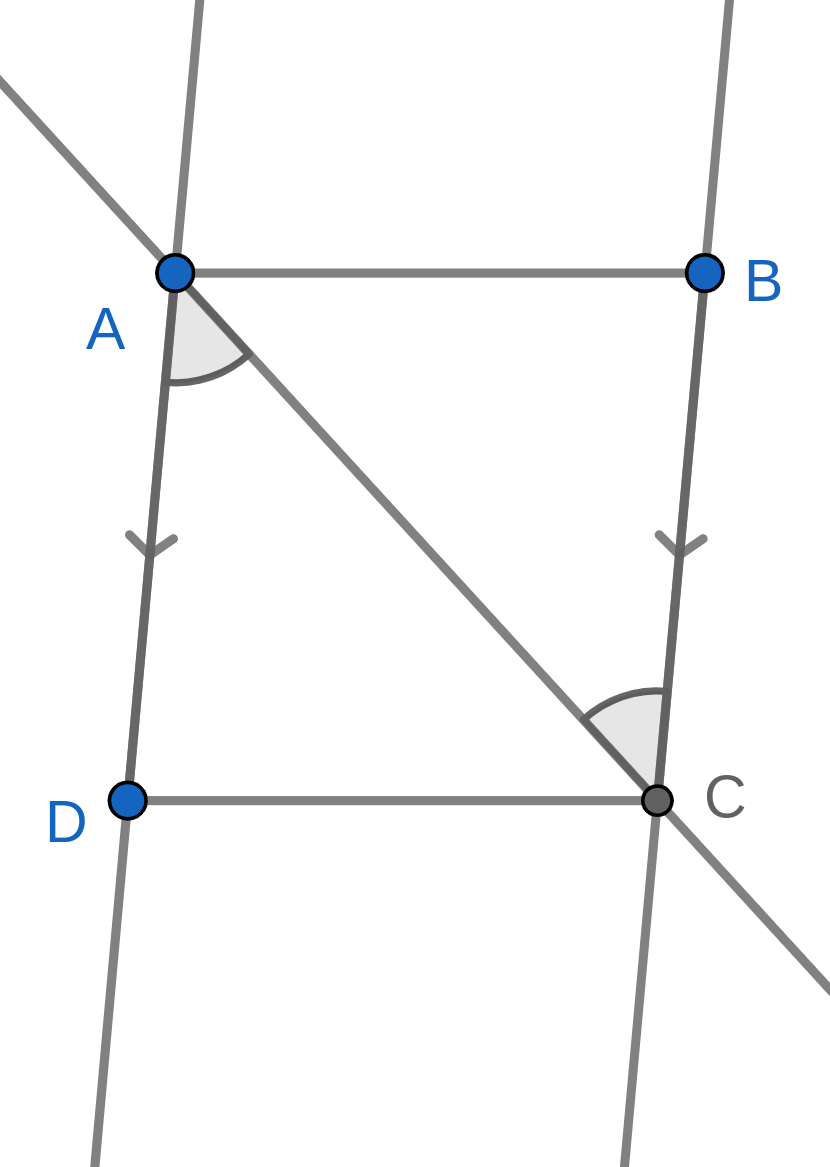
\includegraphics{images/rhombus_parallel_sides.png}
\end{marginfigure}

By Corollary \ref{corollary:rhombus-angle-bisectors}, we see that $AC$ divides the rhombus into a pair of congruent isosceles triangles: triangle $ABC$ and triangle $ADC$. We conclude that angle $BCA$ is congruent to angle $DAC$.

This means that the line $AC$ falls upon the lines $AB$ and $CD$ in such a way as to make the alternate interior angles congruent. By Euclid's Proposition I.27, the lines $AB$ and $CD$ are parallel.

One argues for the other pair of sides in an entirely similar manner, but using angles $BAC$ and $ACD$ instead.
\end{proof}


\begin{corollary}[Conjecture 1.1]\label{corollary:rhombus-rigidity}
Let $ABCD$ be a rhombus. If angle $BAC$ is congruent to angle $BDC$, then $ABCD$ is a square.
\end{corollary}

\begin{proof}
By Corollary \ref{corollary:rhombus-angle-bisectors}, adding the diagonal $AC$ divides the rhombus $ABCD$ into a pair of congruent isosceles triangles $ABC$ and $ADC$. In particular, the angles $BAC$ and $CAD$ are congruent.

The same argument works for dividing the rhombus with the diagonal $BD$, and we learn that angles $BDA$ and $BDC$ are congruent.

\begin{marginfigure}
  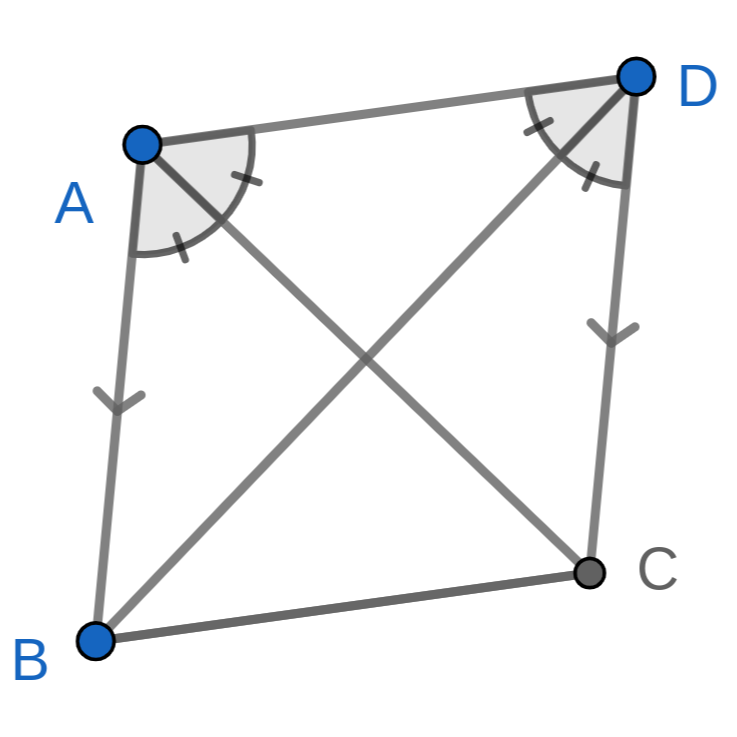
\includegraphics{images/rhombus_rigidity.png}
\end{marginfigure}

By our hypothesis, this means that all four of the angles $BAC$, $ACD$, $BDA$, and $BDC$ are congruent. Gathering these together in pairs which share a side, and using the fact that sums of equals must be equal, we see that angle $BAD$ is congruent to angle $ADC$.

But since $ABCD$ is a parallelogram, the lines $AB$ and $DC$ are parallel. Note that the line $AD$ falls upon them with the angles $BAD$ and $ADC$ being the pair of interior angles on the same side. So by Euclid's Proposition I.29, these angles taken together make two right angles. Since they are congruent and together make two right angles, each must be a right angle.

Looking closer, we see that each of the angles $BAC$, $ACD$, $BDA$, and $BDC$ is congruent to half a right angle.
By Euclid's proposition I.5, the same must be true for the angles $BCA$, $ACD$, $ABD$, and $DBC$. Gathering these together in pairs which share a side, we learn that angles $ABC$ and $BCD$ are right angles.

Since $ABCD$ is a quadrilateral having four mutually congruent sides and four right angles, it is a square.
\end{proof}


\begin{theorem}[Conjecture 1.7]\label{theorem:rhombus-diags-perp}
Let $ABCD$ be a rhombus, if the segments $AC$ and $BD$ meet at a point $X$, then $AXB$ is a right angle.\sidenote{One can get more out of this: the two diagonals divide the rhombus into four right triangles which are all mutually congruent.}
\end{theorem}

\begin{proof}
Let $ABCD$ be a rhombus for which the segments $AC$ and $BD$ meet at a point $X$. Consider the two triangles $AXB$ and $AXD$. We want to show that these triangles are congruent.

\begin{marginfigure}
  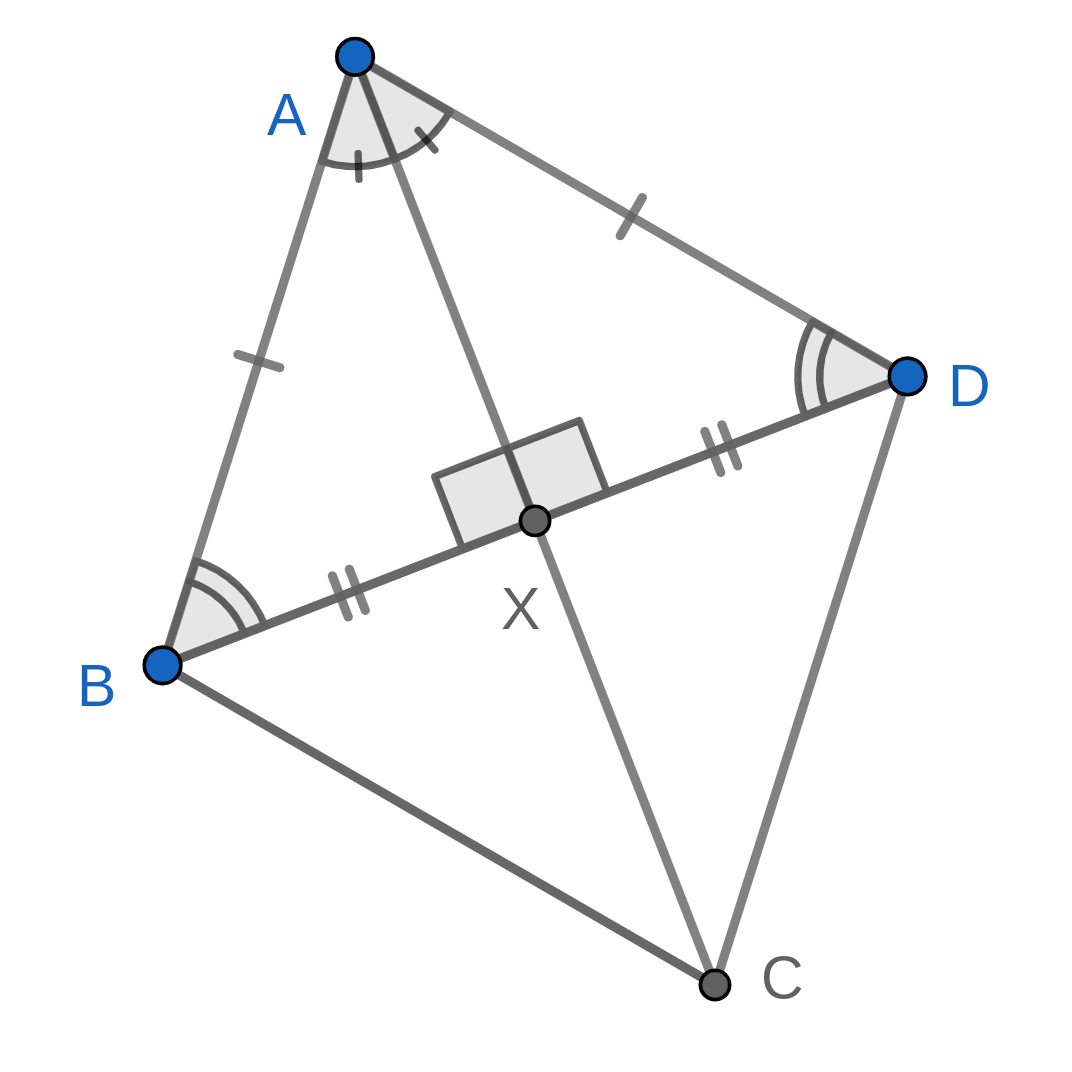
\includegraphics{images/rhombus_diags_perp.png}
\end{marginfigure}

Since $ABCD$ is a rhombus, the segments $AB$ and $AD$ are congruent. We deduce that triangle $BAD$ is isosceles and hence that angle $XBA = DBA$ is congruent to angle $XDA = BDA$ by Euclid's Proposition I.5. By Corollary \ref{corollary:rhombus-angle-bisectors} $AC$ is an angle bisector of angle $BAD$, so angle $BAX$ is congruent to angle $DAX$. So by Euclid's Proposition I.26, triangle $AXB$ is congruent to triangle $AXD$.

In this pair of congruent triangles, the angles $AXB$ and $AXD$ correspond. Also, these two angles are formed by the inclination of the line $AC$ through the line $BD$ at the point $X$, so by Euclid Proposition I.13, these angles either are two right angles, or taken together make as much as two right angles. As these angles are equal, we see that each must be a right angle. In particular, $AXB$ is a right angle.
\end{proof}



\begin{theorem}[Conjecture 1.2]\label{theorem:rhombus-diags-meet}
Let $ABCD$ be a rhombus. Then the diagonal segments $AC$ and $BD$ intersect.
\end{theorem}

\begin{proof}
We have seen that $ABCD$ is necessarily a parallelogram, so by Euclid's Proposition I.29, the angles $BAD$ and $CDA$ taken together make two right angles. We have proved that the diagonal $AC$ is the angle bisector of angle $BAD$ and the diagonal $BD$ is the angle bisector of angle $CDA$. Therefore, the angles $CAD$ and $BDA$ taken together are half of two right angles, which is certainly less than two right angles.

\begin{marginfigure}[-0.75in]
  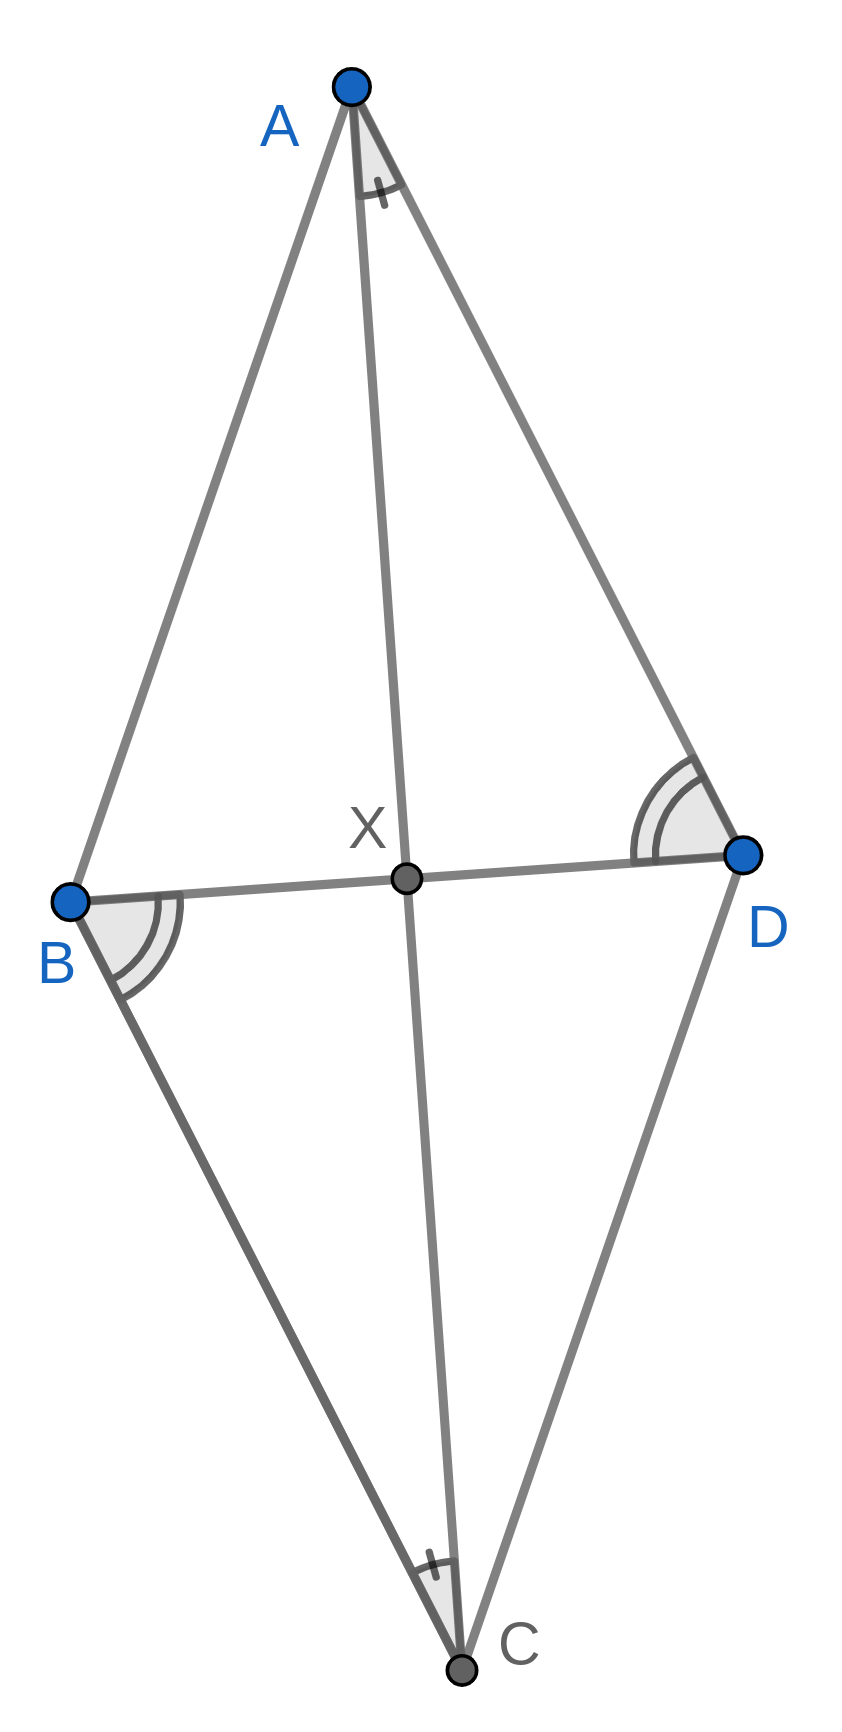
\includegraphics{images/rhombus_diag_meet.png}
\end{marginfigure}

So, by Euclid's Postulate 5, the rays $AC$ and $BD$ meet at some point $X$. By the statement of Postulate 5, $A$ does not lie between $C$ and $X$ in line $AC$. Similarly, $B$ does not lie between $D$ and $X$ on line $BD$.\sidenote{One set of axioms which is needed but appears only implicitly in Euclid's work is a collection of ideas and methods for dealing with \emph{between-ness}. In this case, we need the notion of what it means for one point on a line to lie between two other points on that line.}

Let's repeat the argument, but now working at the vertices on the opposite side $BD$. Following the same arguments, we see that the rays $CA$ and $DB$ meet at some point $Y$, which is situated so that $C$ does not separate $A$ and $Y$ in line $AC$ and $D$ does not separate $B$ and $Y$ in $BD$.

Now, the two lines $AC$ and $BD$ are different, so they can meet only once.\sidenote{Here is another unnoticed axiom!} This means that $X$ and $Y$ are the same point. Also, we learn that $X$ lies between $A$ and $C$ on line $AC$, and hence in the \emph{segment} $AC$. Similarly $X$ lies in the \emph{segment} $BD$.

We deduce that the diagonal segments $AC$ and $BD$ intersect.
\end{proof}

\clearpage

\begin{proof}[Alternate Proof of Theorem \ref{theorem:rhombus-diags-meet}]
Consider the rhombus $ABCD$ with diagonal $BD$. By Euclid's Proposition I.10, we may construct the midpoint $M$ of segment $BD$, so that $BM$ is congruent to $MD$. We shall first show that the triangles $ABM$ and $ADM$ are congruent.

\begin{marginfigure}
  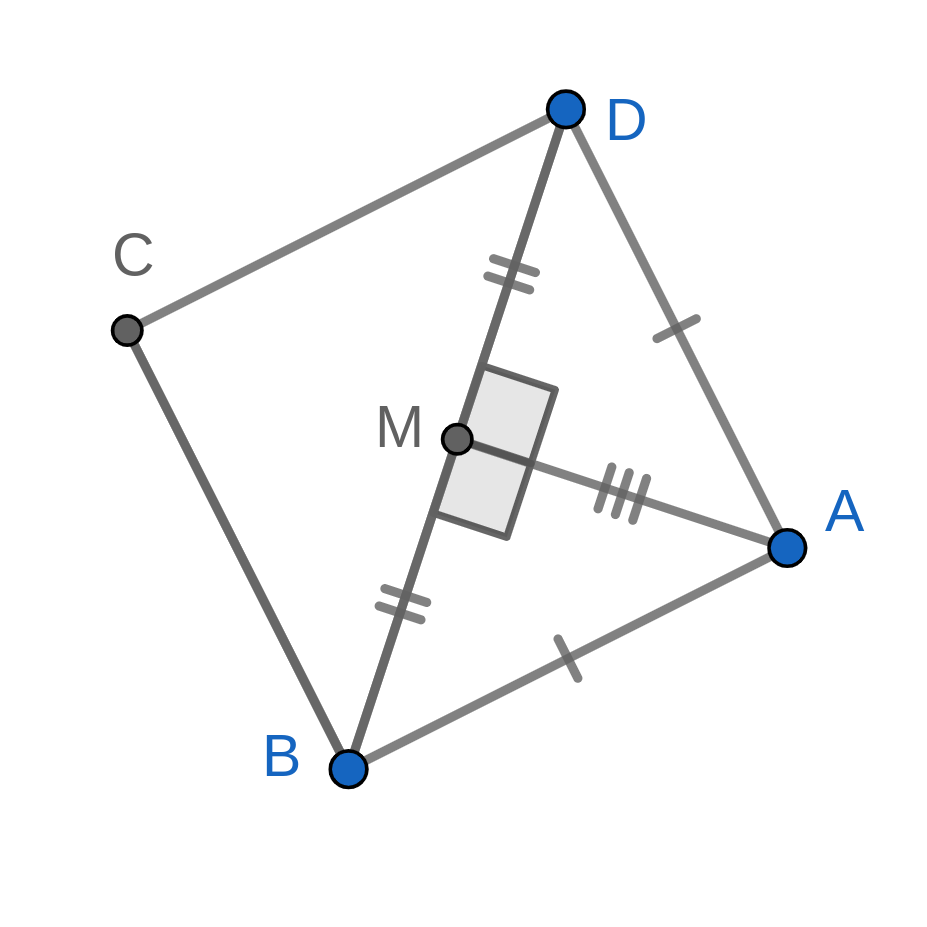
\includegraphics{images/rhombus_midpt_diag_pf.png}
\end{marginfigure}

Note that since $ABCD$ is a rhombus, the segments $AB$ and $AD$ are congruent. By construction of the point $M$, the segments $BM$ and $DM$ are congruent. Finally, the segment $MA$ is common to both triangles, and is congruent to itself. So by Euclid's Proposition I.8, the triangles $ABM$ and $ADM$ are congruent.

Since corresponding parts of congruent triangles are congruent, we deduce that angle $BMA$ is congruent to angle $DMA$. But these angles are the result of the straight line $AM$ being set up on the straight line $BD$, so by Euclid's Proposition I.13 these angles must either be two right angles, or taken together must make as much as two right angles. Since our angles are congruent, they must each be a right angle.

We can make exactly the same arguments as above with the triangles $CBM$ and $DBM$. We deduce that the angles $DMC$ and $BMC$ are also right angles.

We are now in the situation of Euclid's Proposition I.14, where the two lines $AM$ and $CM$ lie on opposite sides of the line $BD$, and make angles which taken together make two right angles. We conclude that $AM$ and $CM$ are parts of a single line. This means that $A$, $M$ and $C$ are collinear.

Now we know that the segment $AC$ meets the segment $BD$ at the midpoint $M$ of $BD$. In particular, these segments intersect.
\end{proof}

We dropped an extra axiom in one of the arguments for this last theorem. Let's make it explicit.

\begin{postulate}[Uniqueness of Lines]
Two lines can meet at most once. That is, if two lines share at least two distinct points, then the lines are equal.
\end{postulate}




\clearpage


%%%%%%%%%%%%%%%%%%%%%%%%%%%%%%%%%%%%%%%%%%%%%%%%%%%%%%
\setcounter{section}{2}
\setcounter{theorem}{0}
\section{The Kite}\label{section:kites}


\begin{theorem}[Conjecure 2.1]\label{theorem:kites-1}
Suppose $ABCD$ is a kite with $AB$ congruent to $BC$ and $AD$ congruent to $DC$. Then angle $BAD$ is congruent to angle $BCD$.
\end{theorem}

\begin{proof}
Construct the diagonal $BD$. We shall show that the the triangles $BAD$ and $BCD$ are congruent.

\begin{marginfigure}
  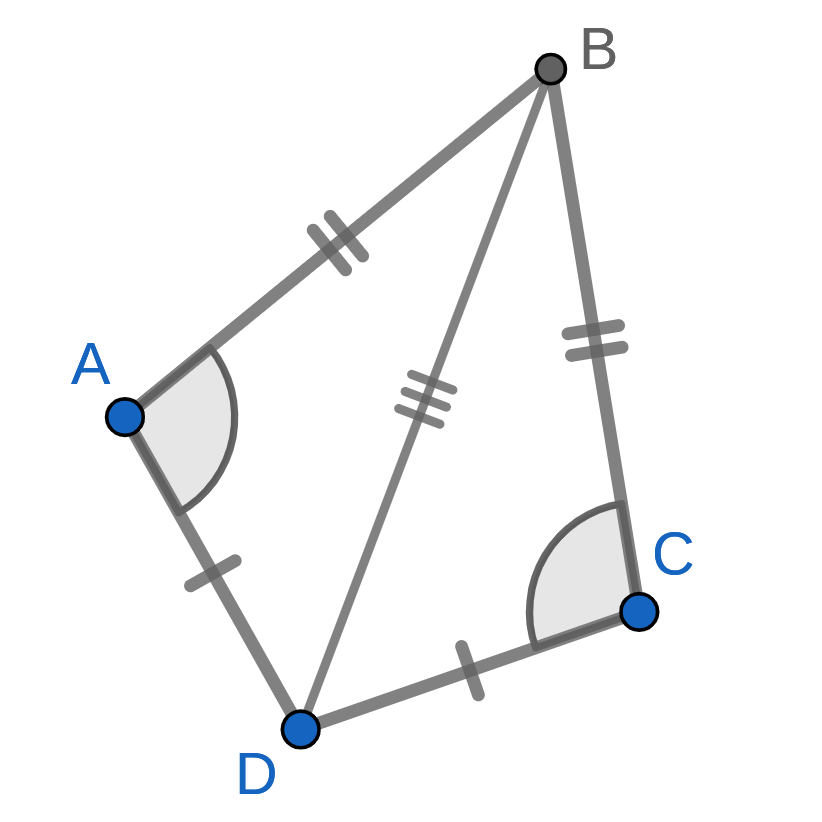
\includegraphics{images/kite_symmetry.png}
\end{marginfigure}


By the hypotheses of the theorem, we know that $AB$ is congruent to $BC$ and $AD$ is congruent to $DC$. The segment
$BD$ is common to both triangles and is congruent to itself. So by Euclid's Proposition I.8, triangle $BAD$ is congruent to triangle $BCD$.

Since corresponding parts of congruent triangles are congruent, we deduce that angle $BAD$ is congruent to angle $BCD$.
\end{proof}

\begin{theorem}[Conjecture 2.1]\label{theorem:kites-2}
There exists a kite with exactly one pair of congruent interior angles.
\end{theorem}

\begin{proof} We shall construct such a kite explicitly.
The idea is to create a special kite using a familiar construction, and then modify it in a way that ensures we get the kinds of angles we know we want. To start, we will follow Euclid's Proposition I.1, and our Theorem \ref{theorem:rhombus-not-square}.

Choose a pair of points $A$ and $C$. Draw circles $AC$ and $CA$. By the Circle-Circle Intersection Property, these two circles meet at two points, let us call them $B$ and $D'$. Draw the segments $AB$, $BC$, $CD'$, and $AD'$. As we have copied the construction in Theorem \ref{theorem:rhombus-not-square}, we know that the quadrilateral $ABCD'$ is a rhombus built out of two equilateral triangles.

\begin{marginfigure}
  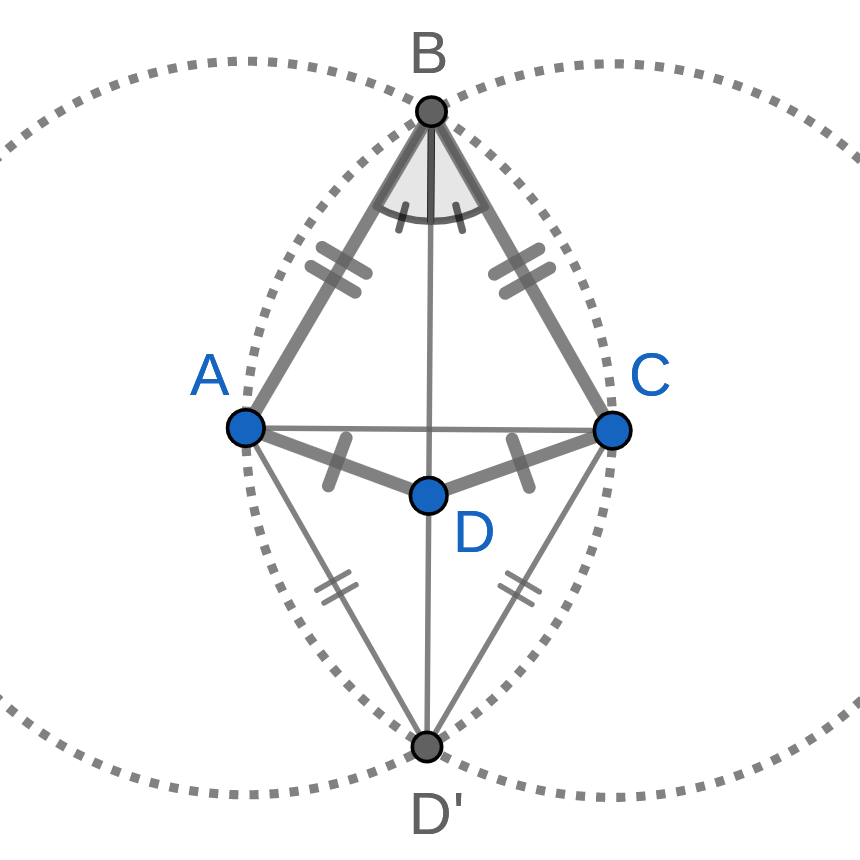
\includegraphics{images/kite_1.png}
\end{marginfigure}

Construct the diagonal segments $BD'$ and $AC$ of the rhombus $ABCD'$, and then choose a point $D$ which lies on the segment $BD'$ and inside triangle $ACD'$. We claim that the figure $ABCD$ is a kite, and that in this kite the opposite angles $ABC$ and $ADC$ are not congruent. The missing pieces are (1) that segment $AD$ is congruent to segment $CD$; and (2) that angle $ADC$ is greater than angle $ABC$.

First, let us prove that $AD$ is congruent to $CD$. By construction, $AB$ is congruent to $BC$ and $AD'$ is congruent to $CD'$. Of course, $BD'$ is congruent to itself, so the triangle $ABD'$ is congruent to the triangle $CBD'$ by Euclid's Proposition I.8. As they are corresponding parts of these triangles, we deduce that angle $ABD'$ is congruent to $CBD'$. But since $B$, $D$ and $D'$ are collinear and in that order, we see that these angles are the same as $ABD$ and $CBD$, respectively. Since $BD'$ is congruent to itself, we deduce from Euclid's Proposition I.4 that the triangles $ABD$ and $CBD$ are congruent. So the corresponding segments $AD$ and $CD$ are congruent by the definition of congruent triangles.

Since we have constructed our figure so that $AB$ is congruent to $BC$ and $AD$ is congruent to $CD$, we know that $ABCD$ is a kite.

\begin{marginfigure}
  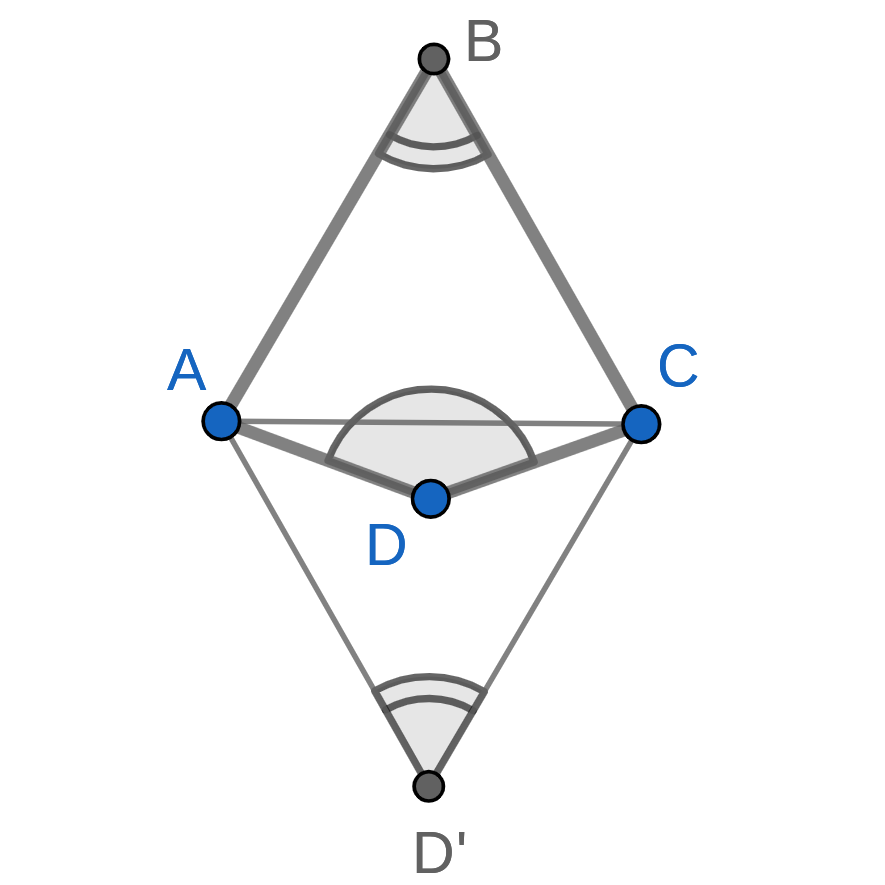
\includegraphics{images/kite_2.png}
\end{marginfigure}


Consider the angle $ADC$. the point $D$ is chosen inside the triangle $AD'C$, by Euclid's Proposition I.21, angle $ADC$ is greater than angle $AD'C$. Now, both angle $ABC$ and angle $AD'C$ are congruent to two-thirds of a right angle by Lemma \label{lemma:rhombus-equilateral-triangles}, hence they are congruent. Therefore, angle $ADC$ is less than angle $ABC$.

So we have constructed the required figure, a kite with a pair of opposite angles which are not congruent.
\end{proof}



\begin{theorem}[Conjecture 2.4] \label{theorem:kites-3}
There is a kite which is not a parallelogram.
\end{theorem}

\begin{proof}
We claim that the kite constructed in the last theorem is not a parallelogram. In particular, the line $AB$ is not parallel to the line $DC$.

By our construction, the angle $ABC$ is two-thirds of a right angle. Similarly, the angles $BCA$ and $CAD'$ are each two-thirds of a right angle. This means that angle $BCD'$ is four-thirds of a right angle. As angle $BCD$ is only part of angle $BCD'$, it is less than four-thirds of a right angle.

\begin{marginfigure}
  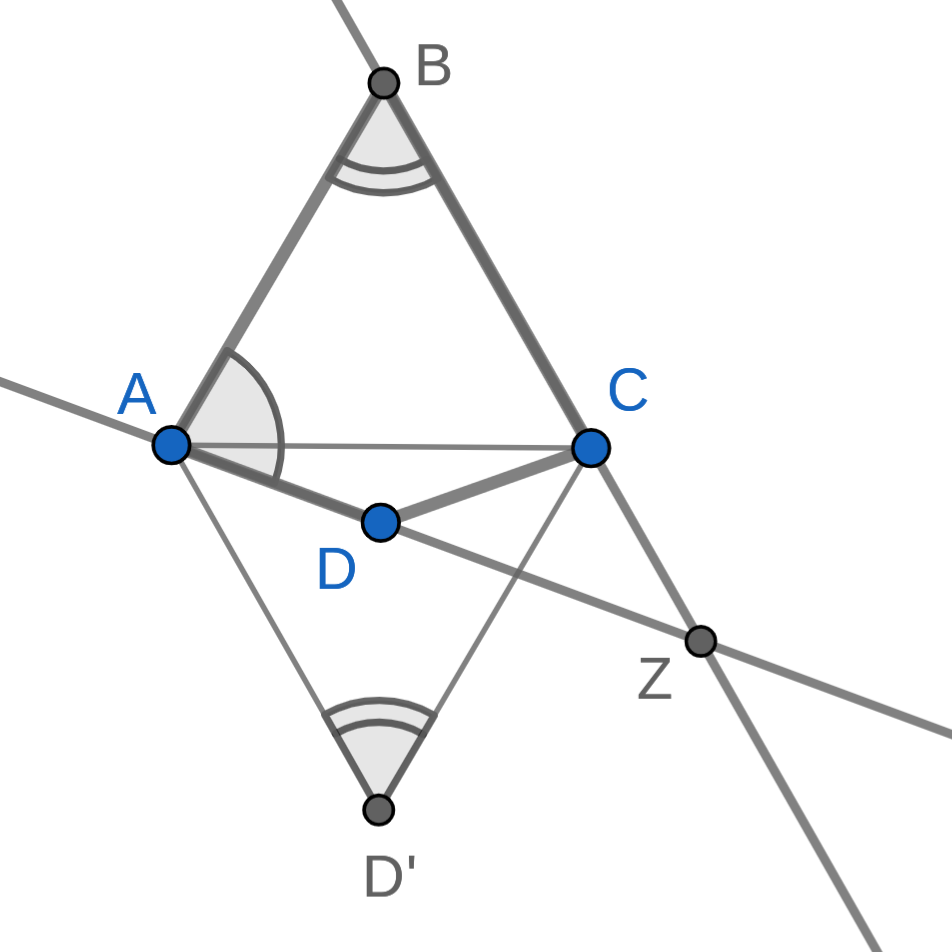
\includegraphics{images/kite_3.png}
\end{marginfigure}

Now focus on the lines $AB$ and $DC$ and the line $BD$ which falls upon them. The interior angles on the side we are considering are $ABC$ and $BCD$, which taken together make less than two right angles. Thus by Euclid's Postulate 5, the lines $AB$ and $CD$ must meet, and are not parallel.
\end{proof}

\begin{theorem}[Conjecture 2.4] \label{theorem:kites-4}
If $ABCD$ is a kite and a parallelogram, then $ABCD$ is also a rhombus.
\end{theorem}

\begin{proof}
Suppose that $ABCD$ is a kite and a parallelogram. Since the figure is a kite, there are two pairs of adjacent and congruent sides. For definiteness, we will say $AB$ is congruent to $BC$ and and $AD$ is congruent to $DC$.



Since $ABCD$ is a parallelogram, by Euclid's Proposition I.34 we deduce that $AB$ is congruent to $CD$ and $BC$ is congruent to $AD$. Therefore, all four sides are mutually congruent. Thus $ABCD$ is a rhombus.
\end{proof}

\clearpage

For our next result, we will want to clear up some language that Euclid uses but does not define.

\begin{definition}\label{definition:same-opp-side}
Let $l$ be a line, and let $X$ and $Y$ be two points which do not lie on $l$. We will say that $X$ and $Y$ \emph{lie on opposite sides of $l$} when the segment $XY$ meets the line $l$. Otherwise, we will say that $X$ and $Y$ \emph{lie on opposite sides of $l$}.
\end{definition}



\begin{theorem}[Conjectures 2.2 \& 2.5]\label{theorem:kites-5}
Suppose that $ABCD$ is a kite. If we extend the diagonals of the kite to lines, then those lines meet. Moreover, those lines must be perpendicular.
\end{theorem}

\begin{proof}
For definiteness, assume our labeling is chosen so that $AB$ is congruent to $BC$ and $AD$ is congruent to $DC$. Construct the line $BD$ using Postulates 1 and 2. By Euclid's Proposition I.7, we deduce that the points $A$ and $C$ cannot lie on the same side of line $BD$. By definition, the segment $AC$ meets the line $BD$.

\begin{marginfigure}
  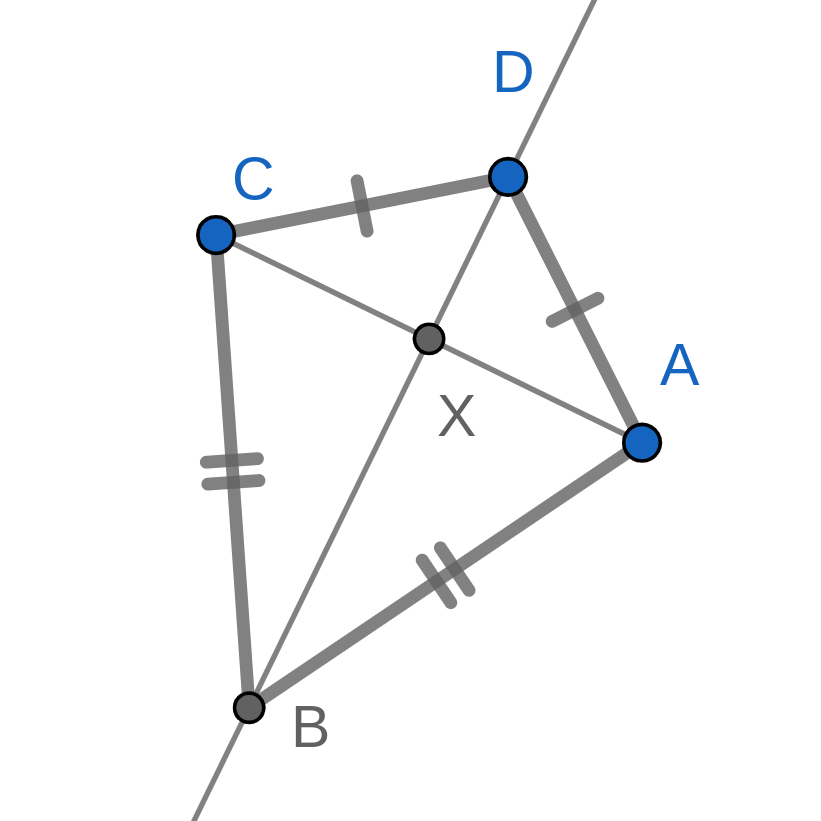
\includegraphics{images/kite_diags_meet_1.png}
\end{marginfigure}

Let us name the point of intersection we just found $X$. Next, we must show that angle $AXB$ is a right angle. Without loss of generality, we assume that the vertices are labeled so that $B$ does not lie between $X$ and $D$. (If it does in a given example, simply switch the roles of $B$ and $D$.)
With this arranged, note that angle $ABX$ is the same thing as angle $ABD$.

Since $AB$ is congruent to $CB$ and $AD$ is congruent to $CD$ and $BD$ is congruent to itself, Euclid's Proposition I.8 guarantees that triangle $ABD$ is congruent to triangle $CBD$. Since these angles correspond, we deduce that angle $ABD$ is congruent to angle $CBD$. Hence, angle $ABX$ is congruent to angle $CBX$.

Now we can see that triangle $ABX$ is congruent to triangle $CBX$ by Euclid's Proposition I.4, since $AB$ is congruent to $CB$, angle $ABX$ is congruent to angle $CBX$, and the common segment $BX$ is congruent to itself.

\begin{marginfigure}
  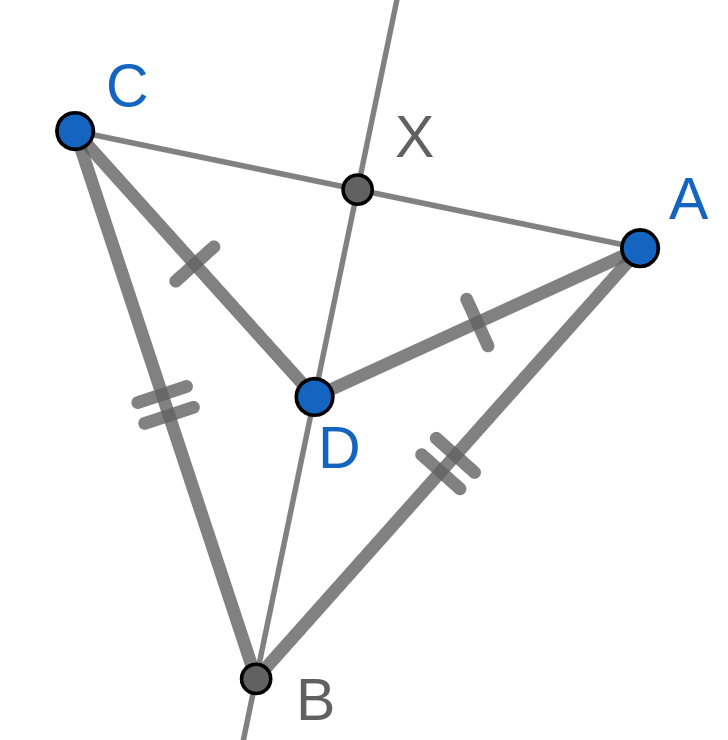
\includegraphics{images/kite_diags_meet_2.png}
\end{marginfigure}


As they are corresponding parts of these congruent triangles, the angles $AXB$ and $CXB$ must be congruent. Further, these two angles are formed by the inclination of the line $XB$ on the straight line $AC$, so by Euclid's Proposition I.13, they are either two right angles or taken together make two right angles. Since they are congruent, each must be a right angle.

Putting it all together, we have proved that the segment $AC$ must intersect the line $BD$ at some point $X$, and the angles formed there must be right angles.
\end{proof}

\clearpage

\begin{theorem}[Conjecture 2.2]\label{theorem:kites-6}
There exists a kite whose diagonal segments do not meet.
\end{theorem}


\begin{proof}
We shall construct such a kite.

We begin by following the construction of a special rhombus as in Theorem \ref{theorem:rhombus-not-square} and Theorem \ref{theorem:kites-2}. To introduce the notation we will need, we repeat the construction in detail. Choose a pair of points $A$ and $C$. By postulate 3 we may construct the circles $AC$ and $CA$. By the Circle-Circle Intersection Property, these circles meet twice. Call the points of intersection $B$ and $E$. The figure $ABCE$ is a rhombus built out of two equilateral triangles which share a side, and hence also a kite.

\begin{marginfigure}
  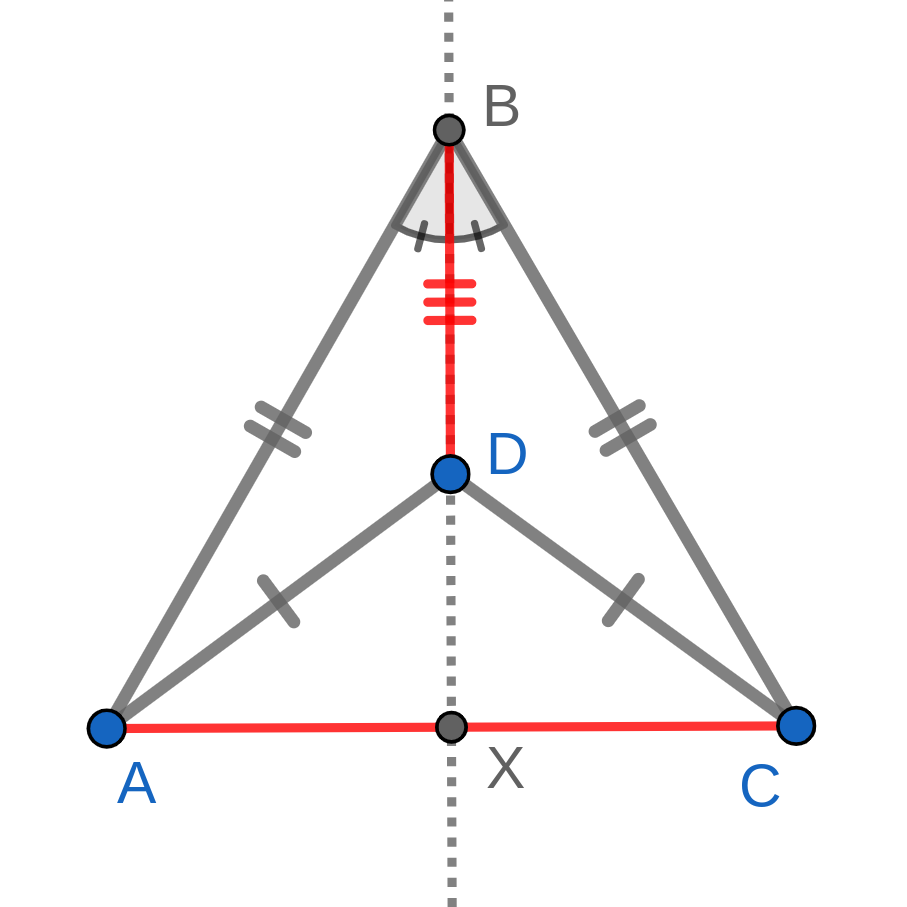
\includegraphics{images/boomerang.png}
\end{marginfigure}


Draw the line $BE$ by Postulates 1 and 2. Draw the segment $AC$ by Postulate 1. By Theorem \ref{theorem:kites-5}, segment $AC$ meets the line $BE$ at some point $X$. Choose a point $D$ which lies on the line $BE$ between the points $B$ and $X$. That is, the new point $D$ lies on the segment $BX$, and hence inside the triangle $ABC$.

Finally, draw in the segments $AB$, $BC$, $CD$, and $DA$. We claim that the figure $ABCD$ is the required kite. The proof that $ABCD$ is a kite proceeds in exactly the same manner as the proof of Theorem \ref{theorem:kites-2}. Since we selected the point $D$ to lie between $X$ and $B$, the points $B$ and $D$ lie on the same side of line $AC$. But the lines $AC$ and $BD$ can meet at most once, and they do meet at $X$, which is not in the segment $BD$. Therefore, the segment $AC$ does not meet the segment $BD$.
\end{proof}




\begin{theorem}[Problem 2.3]
Suppose that $MN$ and $OP$ are given segments, and that $XYZ$ is a given angle. Then there exists a kite $ABCD$ such that $AB$ is congruent to $MN$, $BC$ is congruent to $OP$, and angle $ABC$ is congruent to angle $XYZ$.
\end{theorem}

\begin{proof}
We will construct the required kite. Since it is easiest, we will work directly on top of the given angle $XYZ$. In particular, this means that the point $Y$ will play the role of $B$ in our final construction. If it is required that the resulting kite should lie in some other place, we can use Euclid's Proposition I.3 to place the angle where we want it, and then work as below.

By Euclid's Proposition I.2, we can place a straight line segment congruent to $MN$ with one end on the point $Y$. By Postulate 3, we can draw a circle centered at $X$ with this segment as radius. Where this circle meets the ray $YX$, we obtain a new point $A$.

\begin{marginfigure}
  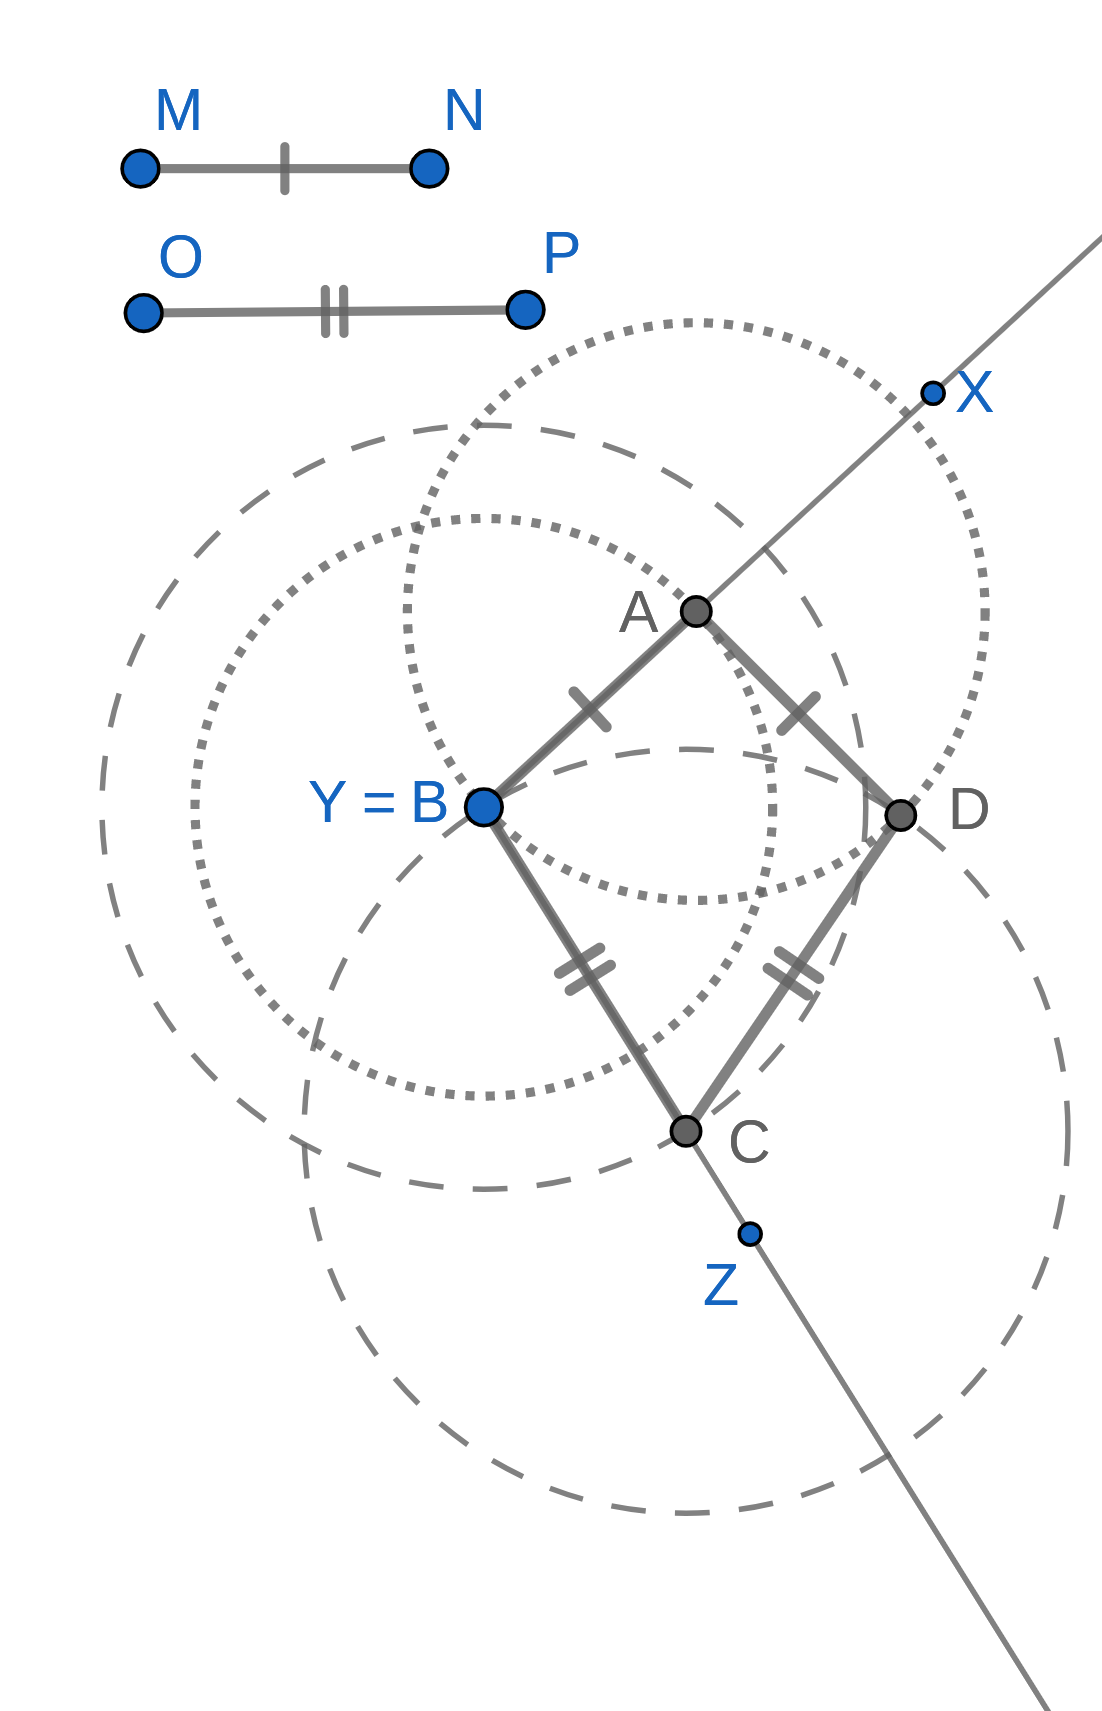
\includegraphics{images/kite_construction.png}
\end{marginfigure}


Similarly, by Euclid's Proposition I.2, we can place a straight line segment congruent to $OP$ with one end on the point $Y$. The by Postulate 3 we can draw a circle with center at $Y$ and with this segment as radius. Where this circle meets the ray $YZ$, we obtain a new point $C$.

Now draw the circles $AB = AX$ and $CB = CX$. These circles meet at $B = X$ by construction. By the Circle-Circle Intersection Property, they meet at two points. Call the other point $D$. Finally, draw the segments $AD$ and $DC$.

By construction the angle $ABC$ is equal to the angle $XYZ$, not just congruent to it. And $AD$ is congruent to $AB$ because they are both radii of the circle $AB$, and $CD$ is congruent to $BC$ because they are both radii of circle $CB$.
Therefore, $ABCD$ is the required kite.
\end{proof}


We seem to use some interesting facts about isosceles triangles repeatedly, so it would benefit us to encapsulate those results in a theorem so we can more readily quote it. Of course, once we get going, we want as much as we can get, so the theorem is rather long. First, we need some new terminology.

\begin{definition}\label{definition:classical-cevians} Let $T$ be a triangle, and let $X$ be a vertex of $T$. The line through $X$ which is perpendicular to the opposite side of $T$ is called the \emph{altitude of $T$ through $X$}.

The line which joins $X$ to the midpoint of the opposite side of $T$ is called the \emph{median of $T$ through $X$}.
\end{definition}



\begin{theorem}[Isosceles Triangle Characterizations] \label{theorem:isosceles-triangle-characterizations}
Suppose that $ABC$ is a triangle. The following things are equivalent:
\begin{enumerate}
\item The triangle is isosceles with $AB$ congruent to $AC$. \item The perpendicular bisector of $BC$ is the same as the angle bisector of angle $BAC$.
\item The perpendicular bisector of $BC$ is the same as the median from $A$.
\item The perpendicular bisector of $BC$ is the same as the altitude from $A$.
\item The altitude from $A$ is the same as the median from $A$.
\item The altitude from $A$ is the same as the angle bisector of angle $BAC$.
\item The angle bisector of angle $BAC$ is the same as the median from $A$.
\end{enumerate}
\end{theorem}

\begin{proof}
There are so many different conditions here that we have many different arguments to give. We will break the proof up into sections to make things easier.

\begin{description}
\item[(1) implies the rest:]
First assume that $AB$ is congruent to $AC$. We will show that in such a triangle all four of the interesting lines described are equal. That will establish that condition (1) implies all of the other six conditions.



By Euclid's Proposition I.10 we may construct the midpoint $M$ of segment $BC$. By definition, $BM$ is congruent to $CM$. Now construct the segment $AM$, which is the median from $A$. Note that $AM$ is congruent to itself. Therefore by Euclid's Proposition I.8, triangle $ABM$ is congruent to triangle $ACM$.

\begin{marginfigure}
  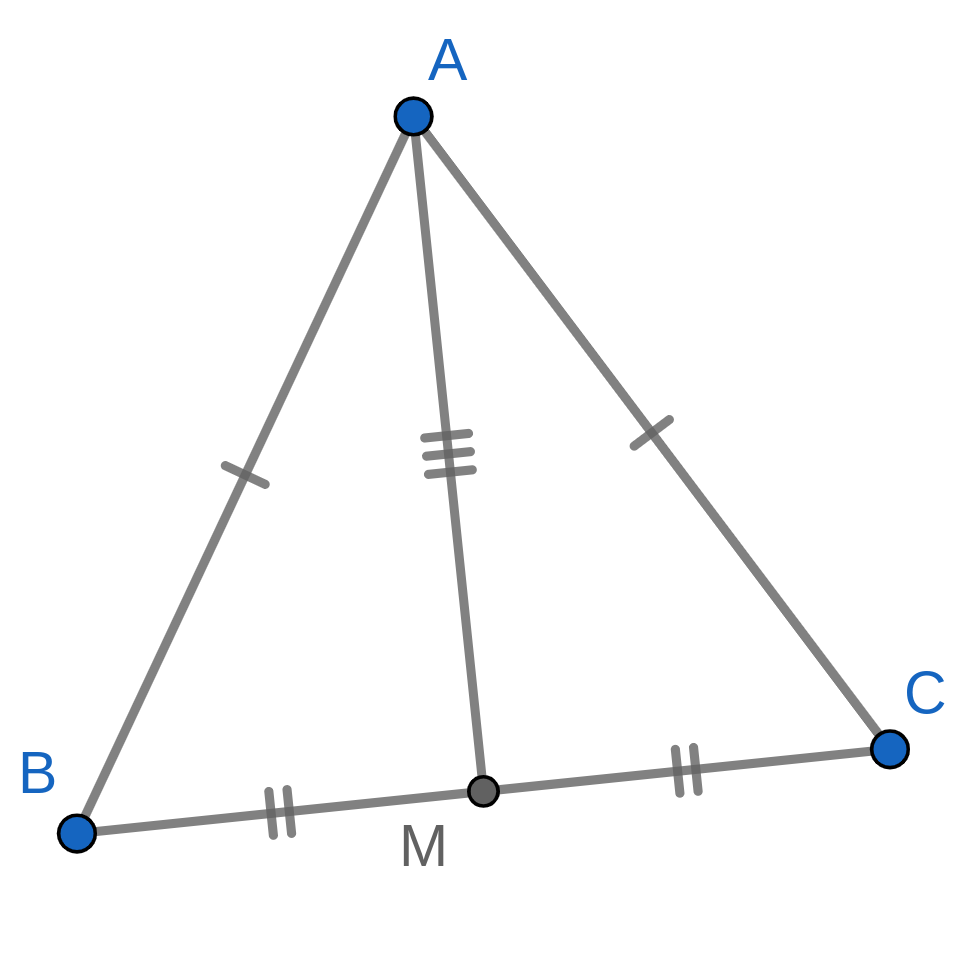
\includegraphics{images/iso_1.png}
\end{marginfigure}


Now, since they are corresponding parts of these two congruent triangles, angle $BAM$ is congruent to angle $CAM$. This means that $AM$ is also the angle bisector of angle $BAC$.



Again, since they are corresponding parts of congruent triangles, angle $BMA$ is congruent to angle $CMA$. These two angles are the result of the inclination of $MA$ on the straight line $BC$, so by Euclid's Proposition I.13 they either make two right angles or angles which taken together make two right angles. Since these angles are congruent, they must each be a right angle. That means that $AM$ is perpendicular to $BC$. Thus $AM$ is also the altitude from $A$, and also the perpendicular bisector of $BC$.

Therefore, if $AB$ is congruent to $AC$ then all of conditions (2) through (7) hold.


\item[each of (2) through (5) implies (1):]
\begin{marginfigure}
  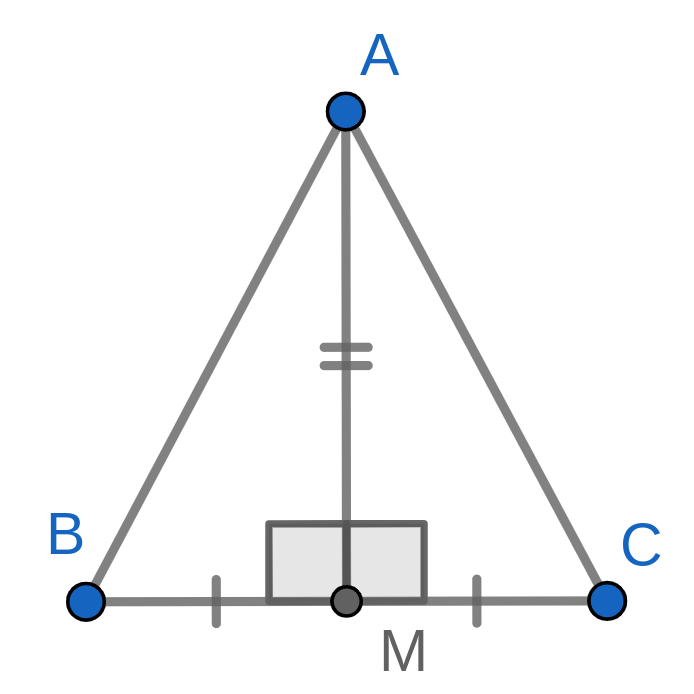
\includegraphics{images/iso_2.png}
\end{marginfigure}
Now we wish to show that each of conditions (2) through (7) implies that $AB$ is congruent to $AC$. This could be very long, but fortunately, there is a significant amount of consolidation.



In any of the situations of (2) through (5) we know the following: The segment $AM$ joins $A$ to the midpoint $M$ of $BC$, and is perpendicular to $BC$. Therefore, we know that $BM$ is congruent to $CM$, angle $BMA$ is congruent to angle $CMA$, and $MA$ is congruent to itself. By Euclid's Proposition I.4, triangle $BMA$ is congruent to triangle $CMA$. Since they are corresponding parts of these triangles, we deduce that $AB$ is congruent to $AC$.


\item[(6) implies (1):]
\begin{marginfigure}
  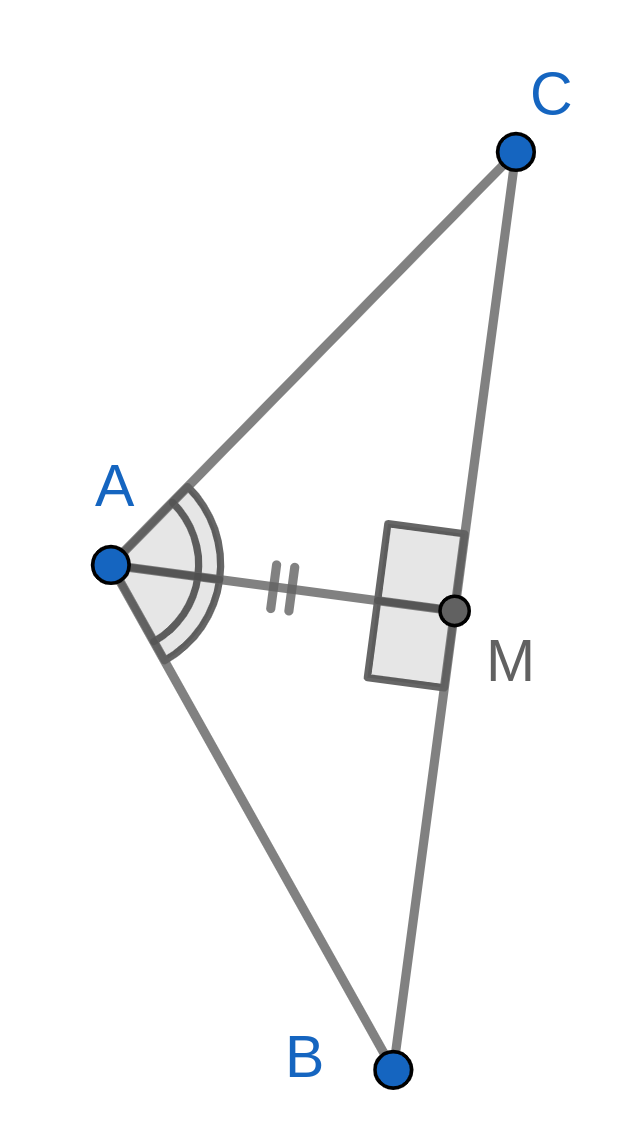
\includegraphics{images/iso_3.png}
\end{marginfigure}
Next, suppose that the altitude from $A$ is the same as the angle bisector of $BAC$. Let the point where the altitude from $A$ meets the line $BC$ be called $M$. Then by construction we know that angle $BAM$ is congruent to angle $CAM$, $AM$ is congruent to itself, and angle $AMB$ is congruent to angle $AMC$ (since they are both right angles). So by Euclid's Proposition I.26, triangle $BMA$ is congruent to triangle $CMA$. Since they are corresponding parts of these triangles, we deduce that $AB$ is congruent to $AC$.

\clearpage

\item[(7) implies (1):]
Finally, we will show that (7) implies (1). This is the most challenging of the  arguments here. Suppose that the angle bisector of $BAC$ is the same as the median from $A$. Then angle $CAM$ is congruent to angle $BAM$, and $CM$ is congruent to $BM$.

We claim that $AM$ is perpendicular to $BC$. That is, we claim that both angle $AMB$ and angle $AMC$ are right angles.

Suppose that $AM$ is not perpendicular to $BC$. By Euclid's Proposition I.13, the angles $AMB$ and $AMC$ taken together make two right angles. Since neither is a right angle, one must be greater and one must be less. Without loss of generality, we assume that $AMB$ is less than a right angle and $AMC$ is greater than a right angle. (If this is not the case, we may run the proof with the letters $B$ and $C$ switched.)


By Euclid's Proposition I.23 we may construct a ray $r$ from the point $M$ so that angle $AMr$ is congruent to the angle $AMB$. Since $AMB$ is less than $AMC$, we know that the ray $r$ lies between the rays $MA$ and $MC$. Therefore, the ray $r$ must cross the segment $AC$. Let the point of intersection be called $B'$.

\begin{marginfigure}
  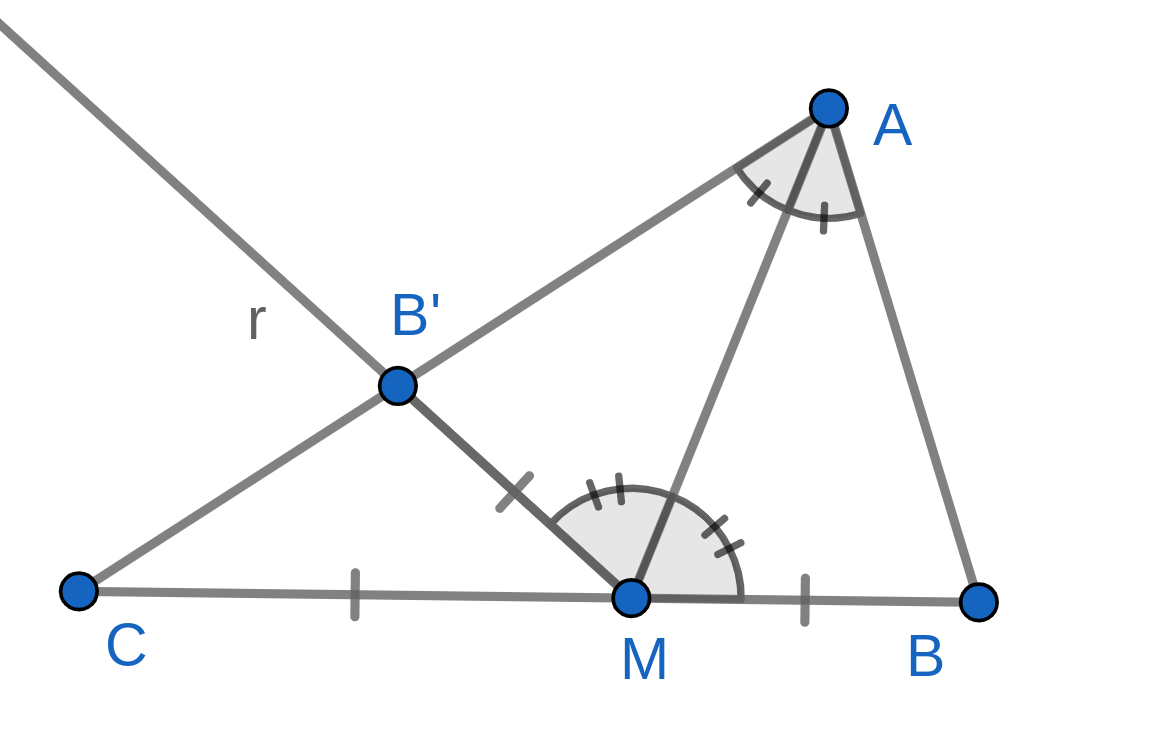
\includegraphics{images/iso_4.png}
\end{marginfigure}


Since angle $CAM = B'AM$ is congruent to angle $BAM$, segment $AM$ is congruent to itself, and angle $AMB$ is congruent to angle $AMB'$, we deduce from Euclid's Proposition I.26 that triangle $AMB$ is congruent to triangle $AMB'$. From this, we deduce that $MB$ is congruent to $MB'$.

Now, we have that $MB$ is congruent to both $MB'$ and $MC$. Therefore, $MB'$ is congruent to triangle $MC$, and the triangle $MCB'$ is isosceles. By Euclid's Proposition I.5, we see that angle $MCB'$ is congruent to angle $MB'C$.

Consider this triangle a bit further. By Euclid's proposition I.32, we know that the three angles of triangle $MCB'$ taken together make two right angles. Since we have just found a pair of them to be congruent, we deduce that twice angle $B'CM$ and angle $CMB'$ taken together make two right angles.

\begin{marginfigure}
  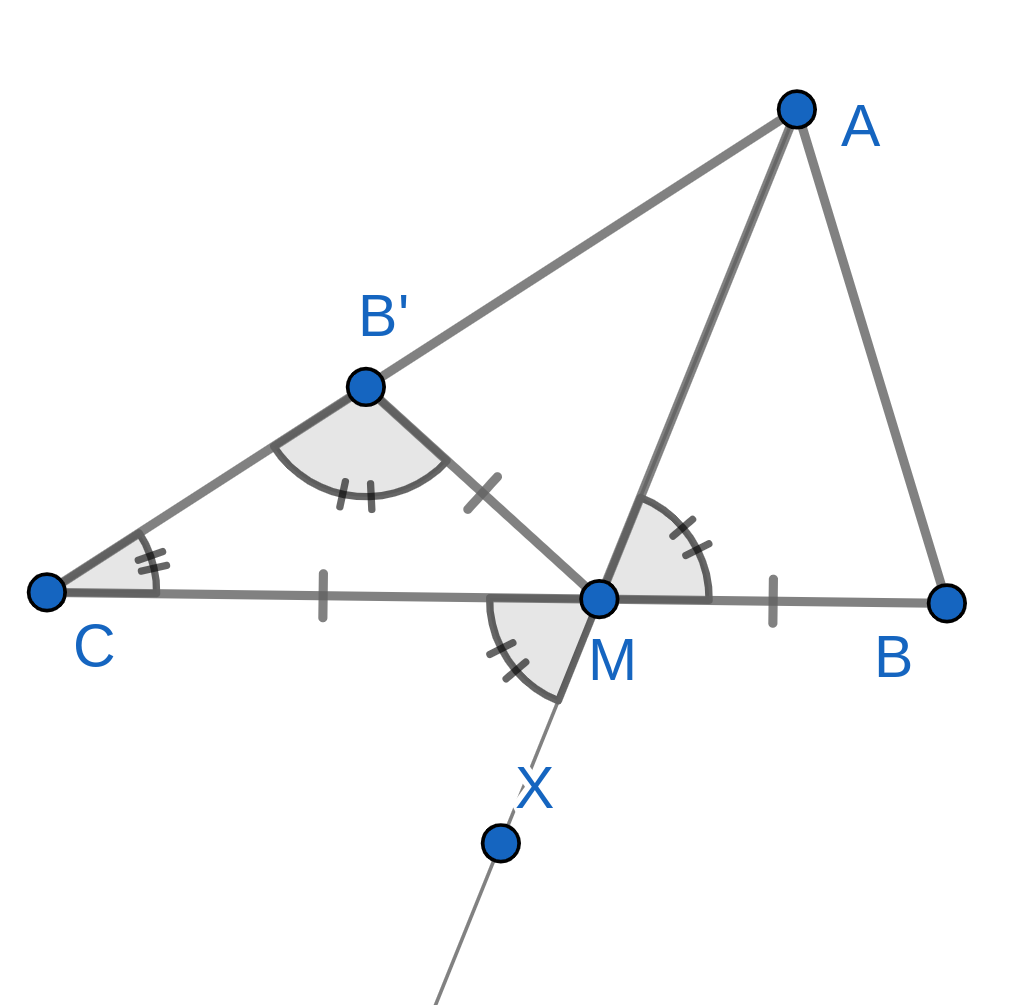
\includegraphics{images/iso_5.png}
\end{marginfigure}

Now reconsider the angles at $M$. We know that angle $CMB'$ and angle $B'MA$ taken together make angle $CMA$. Also, we konw that angle $CMA$ and angle $AMB$ taken together make two right angles. Therefore, the angles $CMB'$, $B'MA$, and $AMB$ taken together make two right angles. But angle $B'MA$ is constructed to be congruent to angle $AMB$, so we learn that
twice angle $AMB$ and angle $CMB'$ taken together make two right angles.

If we now take the conclusions of the last two paragraphs together, we deduce that angle $B'CM$ is congruent to angle $AMB$.



Now extend segment $AM$ to a line, and place a point $X$ on the line so that $M$ lies between $A$ and $X$. By Euclid's Proposition I.15, angle $CMX$ is congruent to angle $AMB$. This means that angle $B'CM$ is congruent to angle $CMX$. These are a pair of alternate interior angles for where the line $CB$ falls on the lines $AC$ and $AM$. By Euclid's Proposition I.27, the lines $AC$ and $AM$ are parallel.

\begin{marginfigure}
  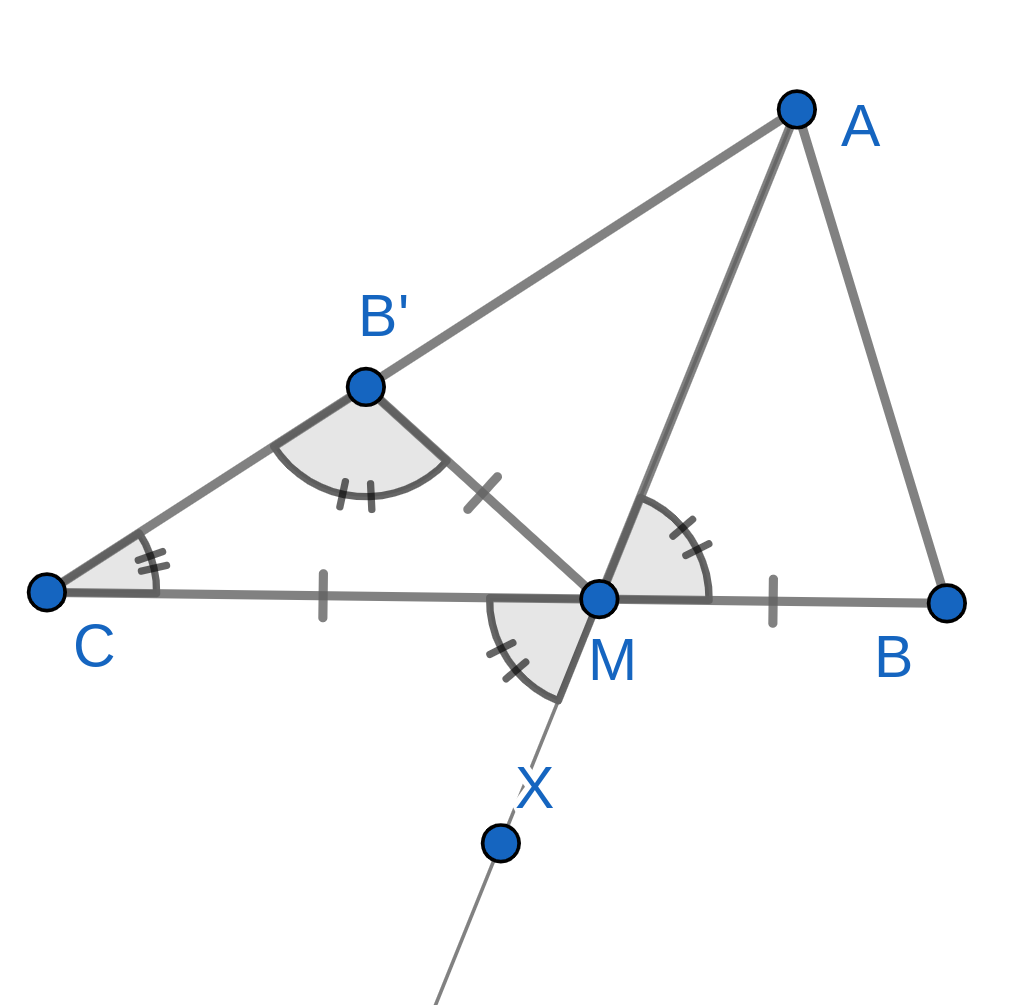
\includegraphics{images/iso_5.png}
\end{marginfigure}

But that is absurd. The lines $AC$ and $AM$ share the point $A$, and hence are not parallel. Since we have arrived at this conclusion by assuming that the angles $AMB$ and $AMC$ are not right angles, it must be the case that these angles are truly right angles. That concludes the argument for the claim.

Now that we know that $AMB$ And $AMC$ are right angles, we see that triangle $BMA$ is congruent to triangle $CMA$. We can use either of Euclid's Proposition I.4 OR Proposition I.26 for this step, as we have two pairs of congruent angles and two pairs of congruent sides, with one of the sides between the angles. Thus, we deduce that $AB$ is congruent to $AC$.
\end{description}
That is the last part of the proof, as we have now demonstrated that each of conditions (2) through (7) is sufficient to deduce condition (1).
\end{proof}


\clearpage

%%%%%%%%%%%%%%%%%%%%%%%%%%%%%%


\section*{Supplement on Convexity, and The Axioms}

We see above that kites come in forms of two distinct characters. It helps to have words to separate the two classes from each other.

\begin{marginfigure}
  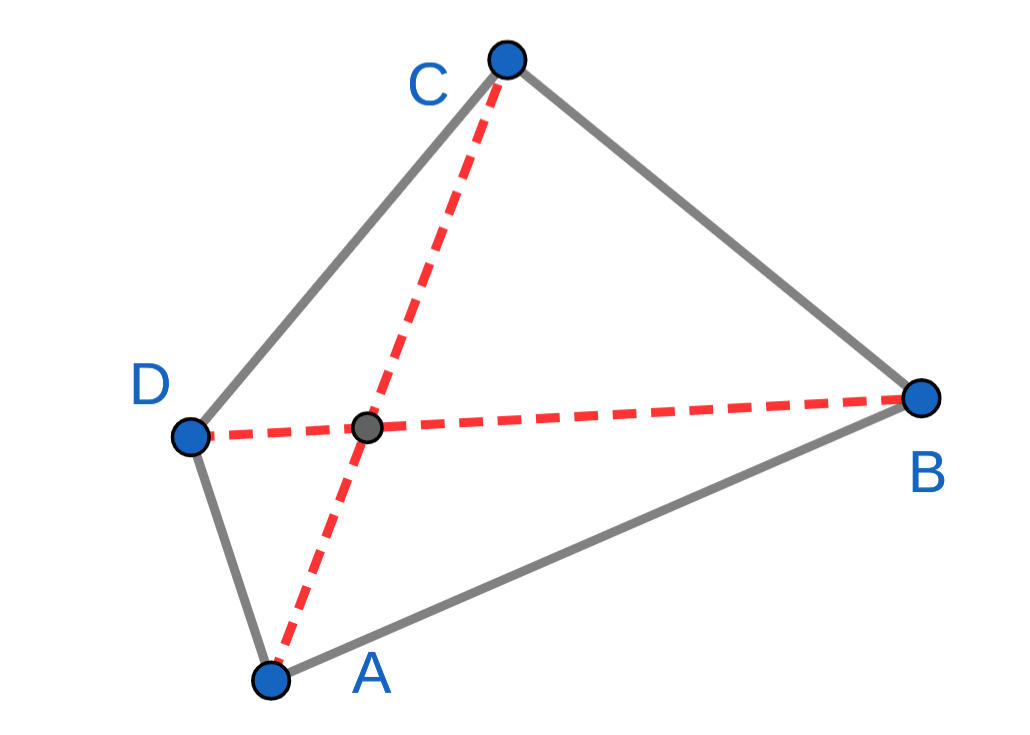
\includegraphics{images/convex.png}
  \caption{A convex quadrilateral}
\end{marginfigure}


\begin{definition}
Suppose that $ABCD$ is a quadrilateral. We will call $ABCD$ \emph{convex} when the diagonal segments $AC$ and $BD$ intersect. We shall call the quadrilateral \emph{non-convex} otherwise.
\end{definition}

\begin{marginfigure}
  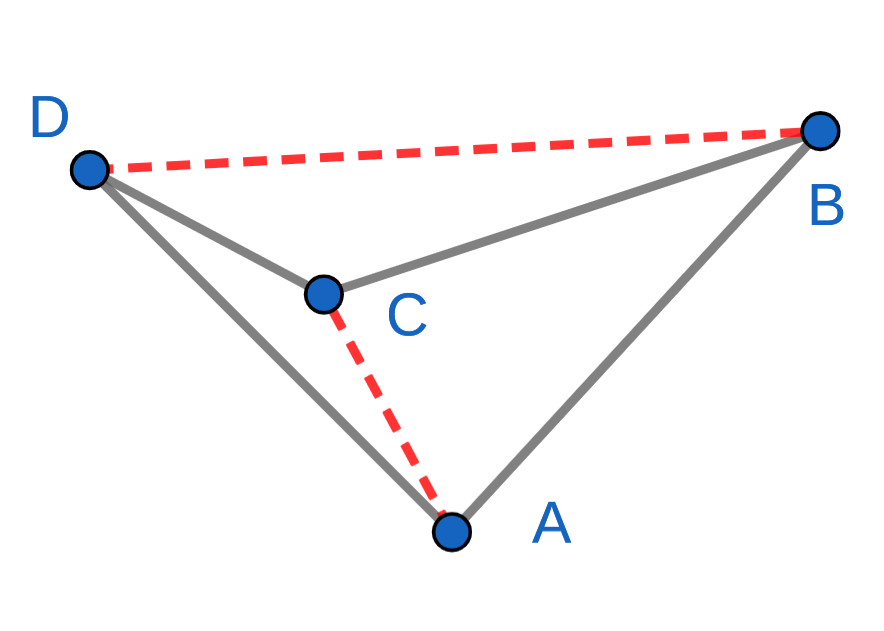
\includegraphics{images/nonconvex.png}
  \caption{A nonconvex quadrilateral}
\end{marginfigure}



In this situation, as in so many others, there are other ways to characterize the property of interest. We can describe convexity for quadrilaterals in several ways, and it is useful and important to know that these ways are logically equivalent. To state the result clearly, we need another new term. To prove the result, we will need several lemmas.


\begin{definition}
Let $X$, $Y$, and $Z$ be three points which are not collinear. We say that a point $P$ \emph{lies inside} the angle $XYZ$ when the points $X$ and $P$ lie on the same side of line $YZ$ and the points $Z$ and $P$ lie on the same side of line $XY$.
\end{definition}


In fact, there is another axiom Euclid does not make explicit that we will want to be careful about.

\begin{postulate}[Triangles are Not Black Holes]
Suppose that $ABC$ is a triangle, and that $\ell$ is a line not containing any of the points $A$, $B$, or $C$. If $\ell$ meets one side of the triangle, then it must also meet one of the other two sides.
\end{postulate}

\begin{marginfigure}
  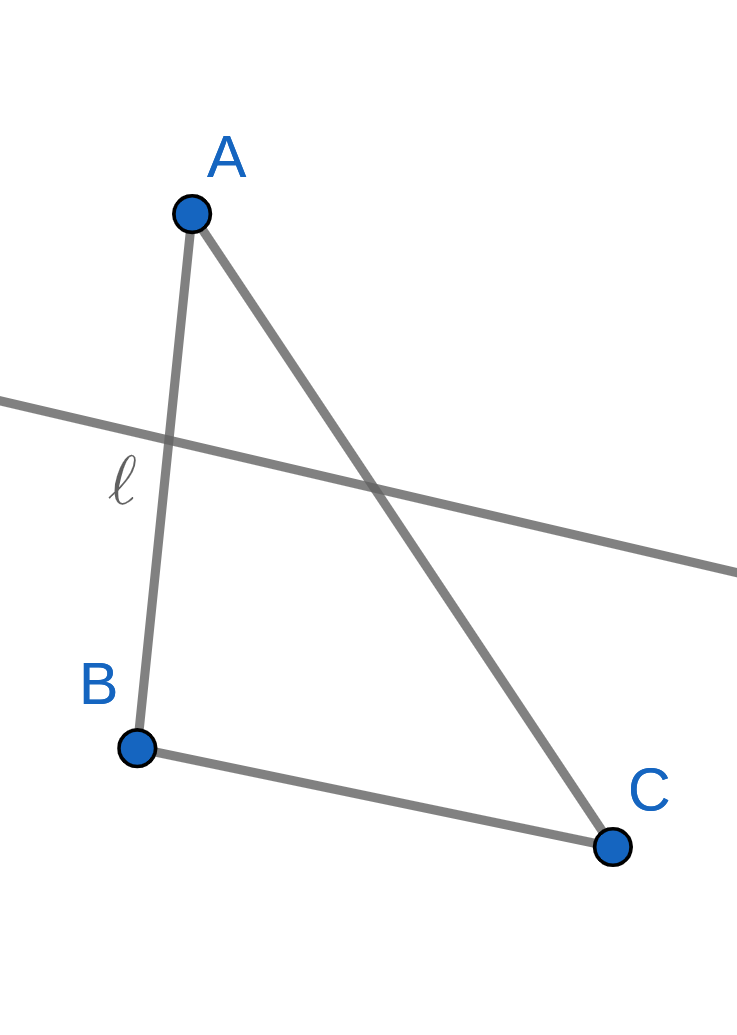
\includegraphics[height=2in]{images/pasch.png}
\end{marginfigure}




\begin{lemma}\label{lemma:same-side-ray}
Let  $\ell$ be a line and $P$ a point on $\ell$. Fix a point $Q$ which is not on $\ell$. If $M$ is a point on the ray $PQ$ different from the point $P$, then $M$ and $Q$ lie on the same side of $\ell$.
\end{lemma}

\begin{proof}
Since $M$ is not equal to $P$, $M$ does not lie on the line $\ell$. Therefore, $M$ either lies on the same side of $\ell$ as $Q$ or on the opposite side of $\ell$. Suppose that $M$ and $Q$ lie on opposite sides of $\ell$. Then the segment $MQ$ meets $\ell$ at some point $X$.

\begin{marginfigure}
  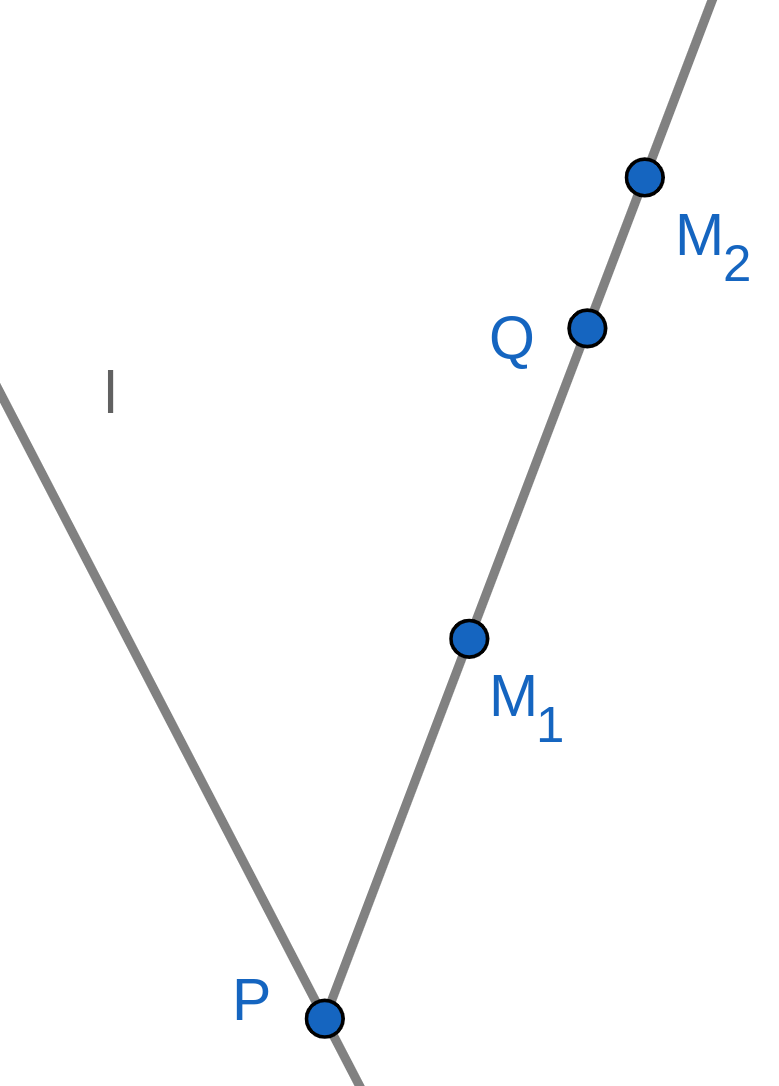
\includegraphics[height=1.5in]{images/oneside.png}
\end{marginfigure}


By construction $P$ does not lie between $M$ and $Q$, so $X$ and $P$ must be different. This means that the line $PQ$ meets the line $\ell$ at two places, namely $P$ and $X$. Since the lines are different, this is impossible. We deduce that $M$ and $Q$ must lie on the same side of line $\ell$.
\end{proof}

This result helps us remove the ambiguity from the next definition. We can read the result of Lemma \ref{lemma:same-side-ray} as saying the choice of point $P$ in the next definition does not matter.

\begin{marginfigure}
  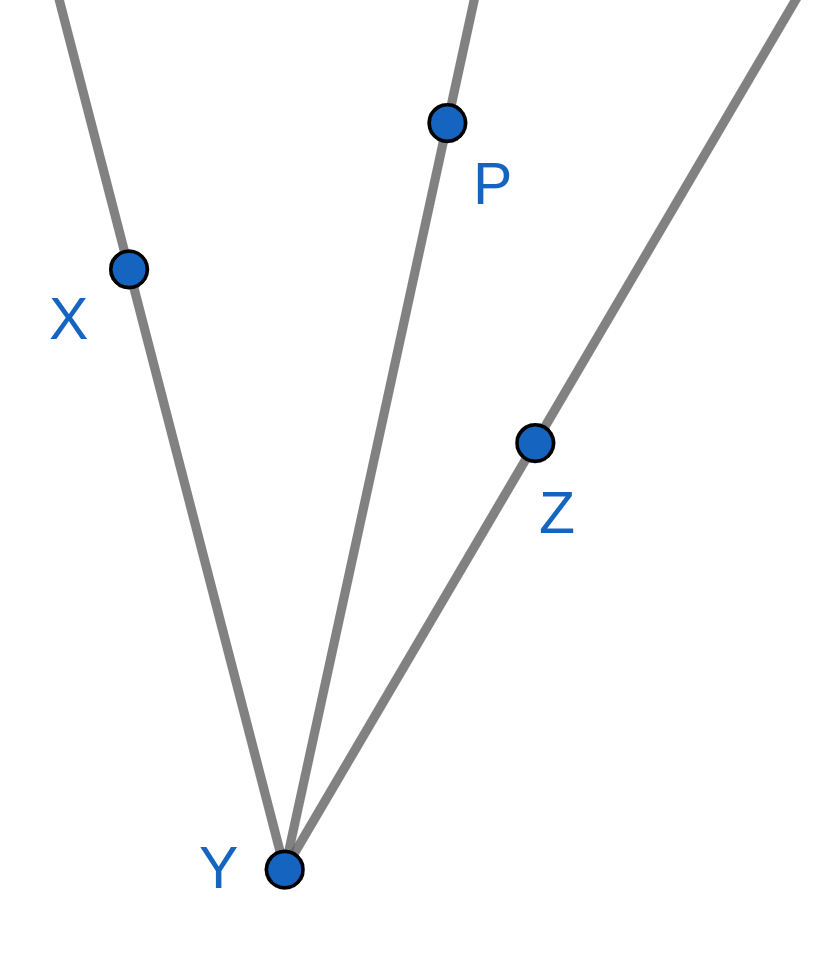
\includegraphics[height=2in]{images/ray_inside_angle.png}
\end{marginfigure}



\begin{definition}
Let $XYZ$ be an angle. We say that a ray $r$ with initial point $Y$ \emph{lies inside angle $XYZ$} if there is a point $P$ on $r$ which is different from $Y$ and lies inside angle $XYZ$.
\end{definition}



\clearpage

\begin{lemma}\label{lemma:same-side-transitive}
Let $\ell$ be a line, and suppose that $X$, $Y$, and $Z$ are three points not lying on $\ell$. If $X$ and $Y$ lie on the same side of $\ell$, and $Y$ and $Z$ lie on the same side of $\ell$, then $X$ and $Z$ lie on the same side of $\ell$.
\end{lemma}

\begin{proof}
Suppose the statement is false, and instead $X$ and $Z$ lie on opposite sides of the line $AB$. Then there exists a point $W$ where the segment $XZ$ meets the line $AB$. But the line $AB$ then crosses the side $XZ$ of the triangle $XYZ$. But a line which meets one side of a triangle must meet at least one of the other two, so $AB$ must also meet either segment $XY$ or segment $YZ$.

\begin{marginfigure}
  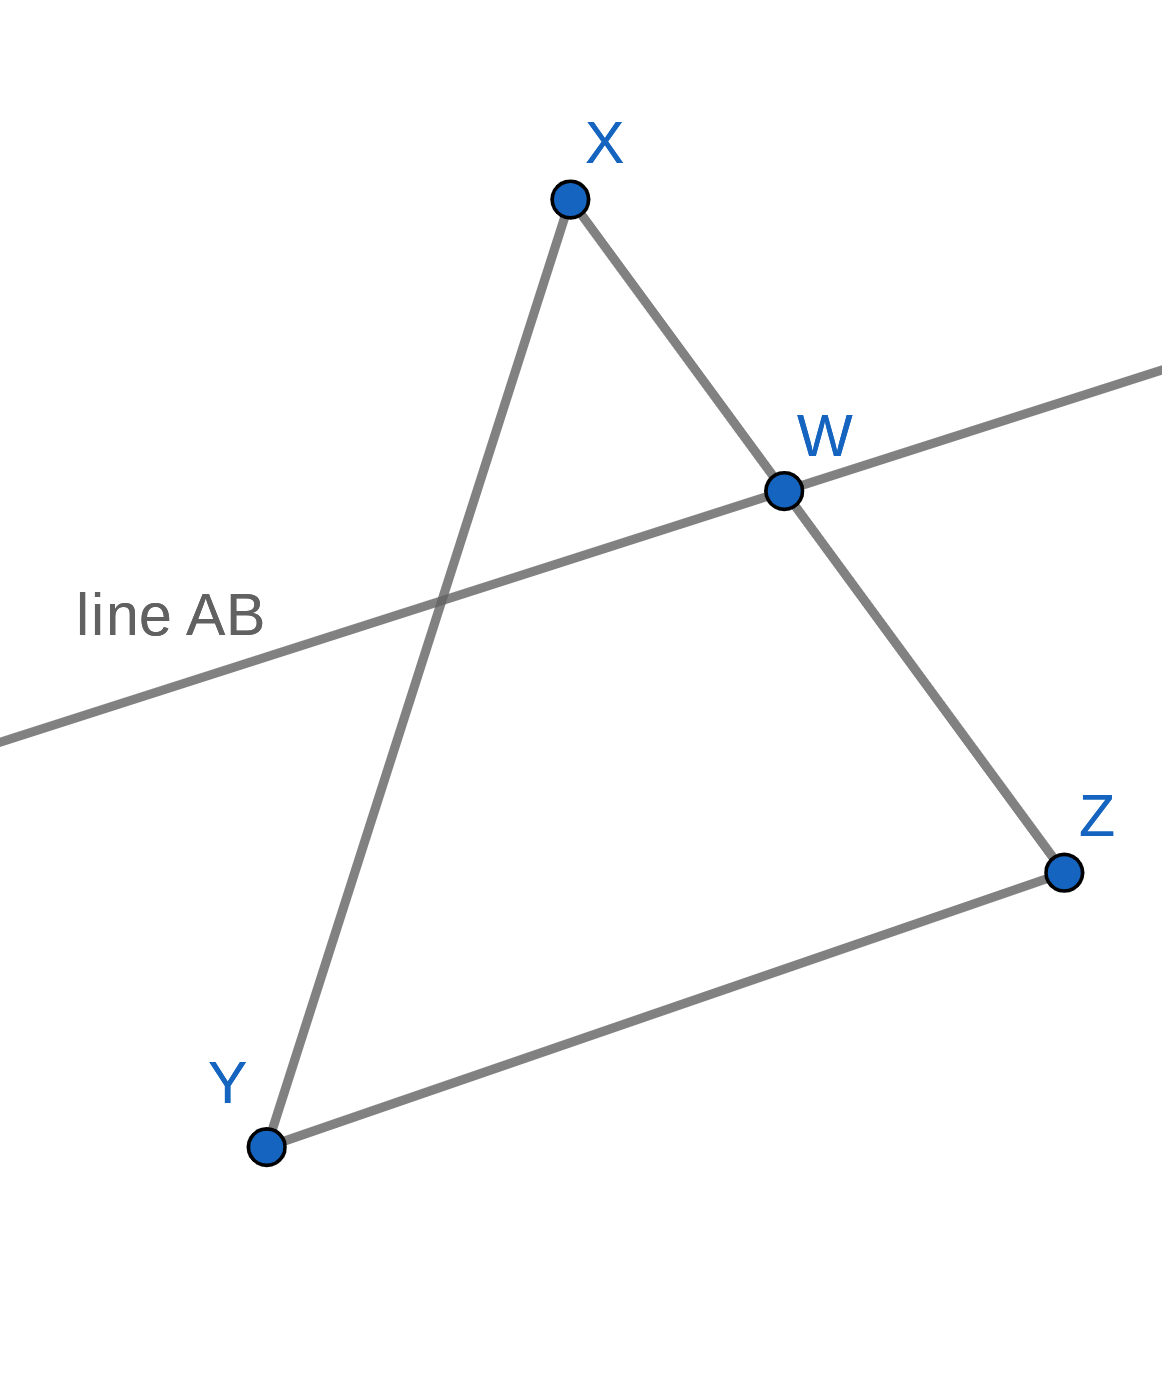
\includegraphics{images/transitive.png}
\end{marginfigure}

Note that since $Y$ does not lie on line $AB$, this line cannot meet both segments $XY$ and $YZ$.
Without loss of generality, assume line $AB$ meets segment $XY$. By definition, this means that $X$ and $Y$ lie on opposite sides of line $AB$. This is contrary to our assumption, so we conclude that $X$ and $Z$ must lie on the same side of line $AB$.
\end{proof}

\begin{definition}
Let $XYZ$ be a triangle. We say a point $P$ \emph{lies inside} $XYZ$ when $A$ and $P$ lie on the same side of $BC$, $B$ and $P$ lie on the same side of $AC$, and $C$ and $P$ lie on the same side of $AB$.
\end{definition}


\begin{lemma}\label{lemma:lighthouse}
Suppose that $XYZ$ is a triangle, and that $P$ is a point inside the triangle $XYZ$. The ray $YP$ meets the segment $XZ$.
\end{lemma}

\begin{proof}
First, we will show that the ray $XP$ meets the ray $YZ$.
Note that angles $XYZ$ and $XZY$ taken together must be less than two right angles by Euclid's Proposition I.17. Since angle $PYZ$ is less than angle $XYZ$, we see that angles $PYZ$ and $XZY$ taken together make less than two right angles. So by Euclid's Postulate 5, the rays $YP$ and $ZX$ must meet at some point $W$.

\begin{marginfigure}
  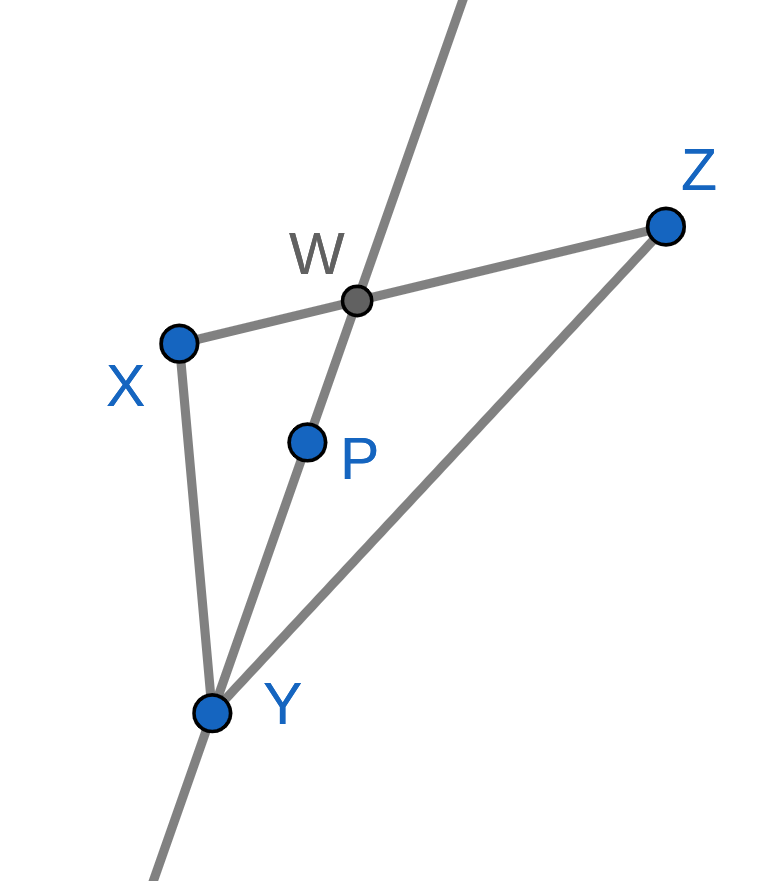
\includegraphics{images/pasch_adjusted.png}
\end{marginfigure}


We claim that $W$ lies between $X$ and $Z$. For if instead $X$ lies between $W$ and $Z$, the angle $PYZ$ would contain the angle $XYZ$. But then $P$ would lie on the opposite side of line $XY$ from $Z$, and therefore not be inside triangle $XYZ$. So we conclude that $W$ lies between $X$ and $Z$ and hence the ray $YP$ meets the segment $XZ$.
\end{proof}


\begin{theorem}[Characterizations of Convex Quadrilaterals]
Suppose that $ABCD$ is a quadrilateral. Use the letters $X$, $Y$, and $Z$ as stand-ins for possible choices of the vertices of the figure. The following conditions are equivalent:
\begin{enumerate}
\item $ABCD$ is convex.
\item For every pair of adjacent vertices $X$ and $Y$, the other two vertices lie on the same side of the line $XY$.
\item For each choice of three consecutive vertices $X$, $Y$, and $Z$ of the quadrilateral, the fourth vertex lies inside the angle $XYZ$.
\end{enumerate}

\end{theorem}

\begin{proof}
There are several steps to this argument. First we shall argue that conditions (2) and (3) are equivalent by showing that (2) implies (3) and then that (3) implies (2). Then we shall prove that (1) and (2) are equivalent by arguing that (1) implies (2), and then finally that (3) implies (1)

\begin{description}
\item[(2) implies (3):] Suppose that a quadrilateral satisfies condition (2). Choose three consecutive vertices of this quadrilateral and call them $A$, $B$, and $C$. We must show that the fourth vertex, call it $D$, lies inside angle $ABC$.

\begin{marginfigure}
  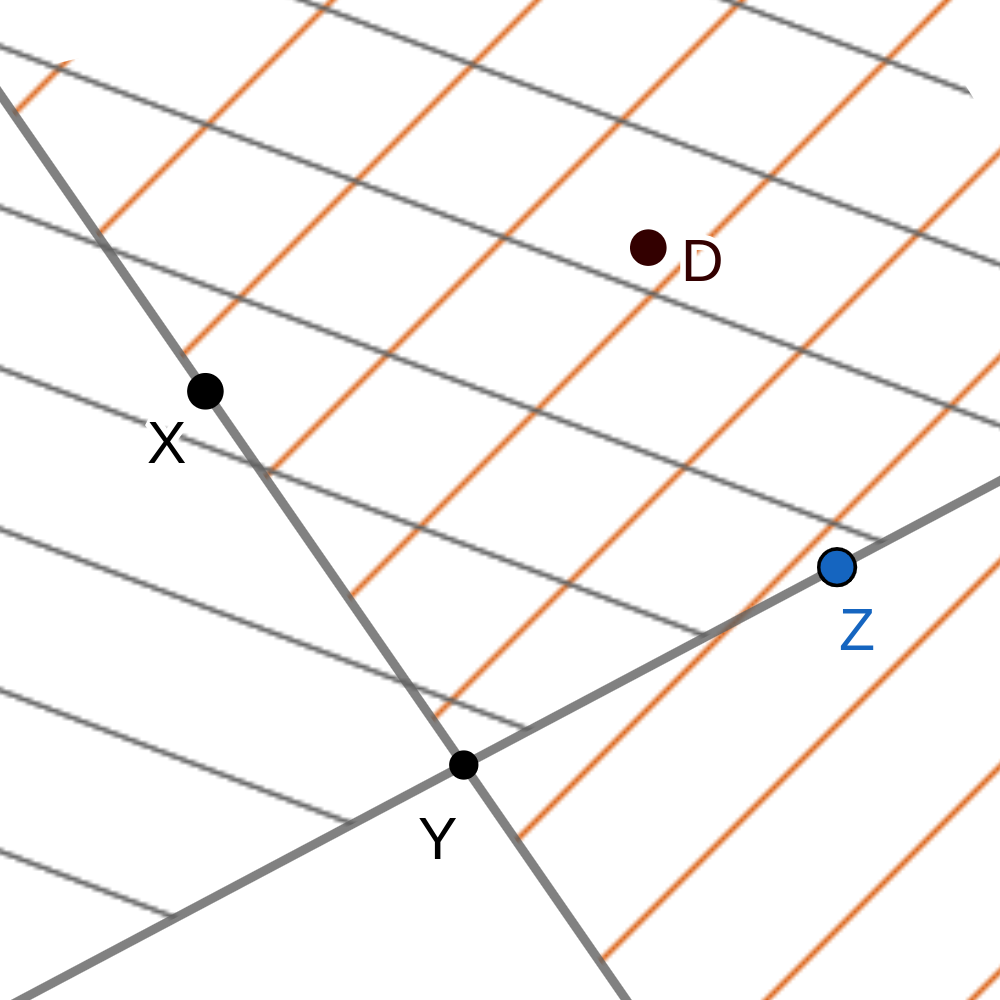
\includegraphics{images/convex_1.png}
\end{marginfigure}


By condition (2), $C$ and $D$ lie on the same side of line $AB$. Also by condition (2), $A$ and $D$ lie on the same side of the line $BC$. By definition, this means that $D$ lies inside angle $ABC$. Since the original choice of three consecutive vertices is made arbitrarily, this holds for all choices of three consecutive vertices. Therefore, condition (3) is true.


\item[(3) implies (2):] Now suppose that our quadrilateral satisfies condition (3). Choose any pair of adjacent vertices $A$ and $B$. We must show that the other two vertices lie on the same side of line $AB$. Without loss of generality, we label these vertices $C$ and $D$, so that the cyclic ordering of vertices in the quadrilateral is $ABCD$.

\begin{marginfigure}
  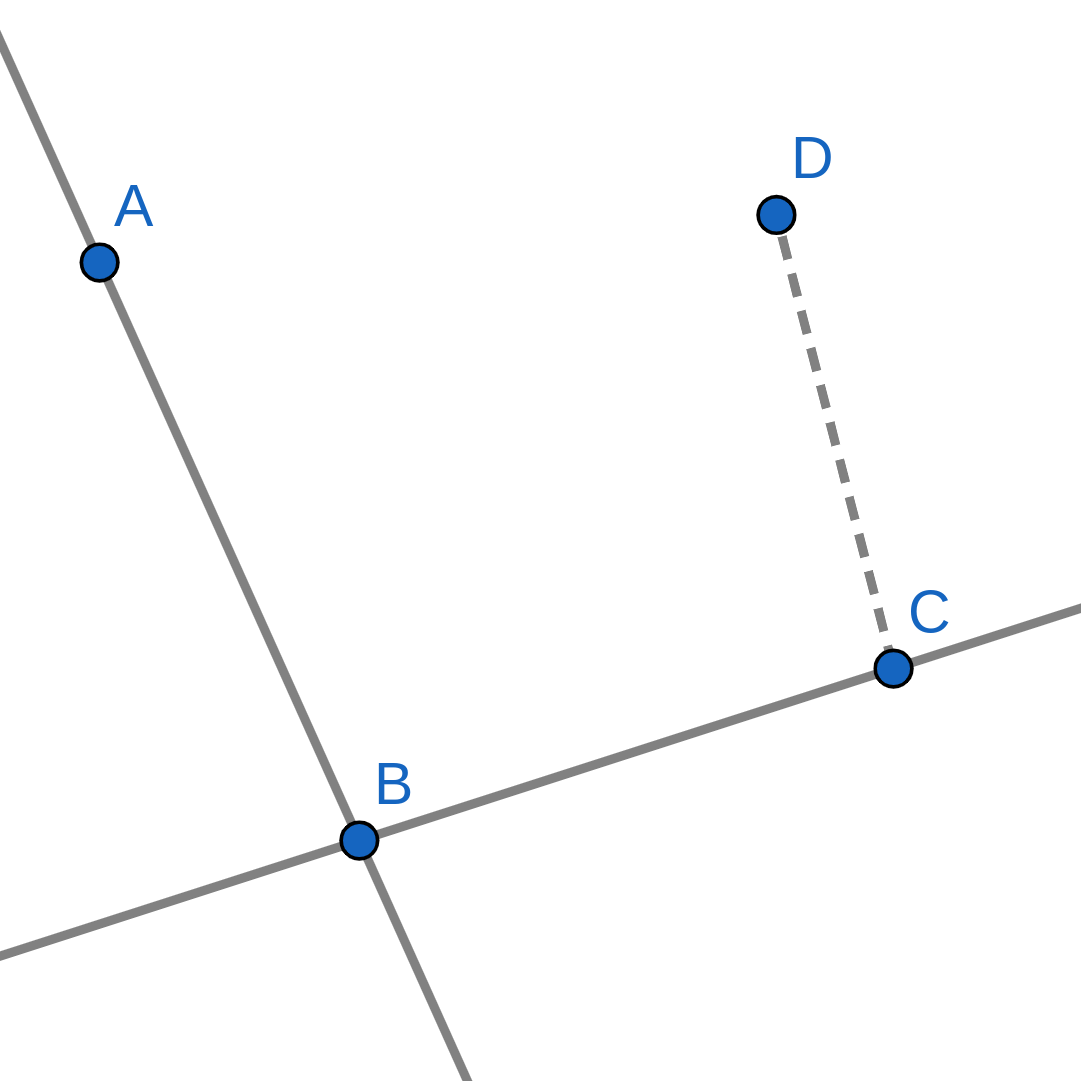
\includegraphics{images/convex_2.png}
\end{marginfigure}

By condition (3), $D$ lies inside the angle $ABC$. By definition, this means that $C$ and $D$ lie on the same side of $AB$, which is what we wanted to prove. Note that our original pair of vertices is chosen arbitrarily, this holds for each pair of adjacent vertices. Therefore, condition (2) is true.

\item[(1) implies (2):] Now suppose that our quadrilateral is convex. We will show that condition (2) is also true. Choose a pair of adjacent vertices $A$ and $B$. We must show that the other two vertices $C$ and $D$ lie on the same side of line $AB$.


\begin{marginfigure}
  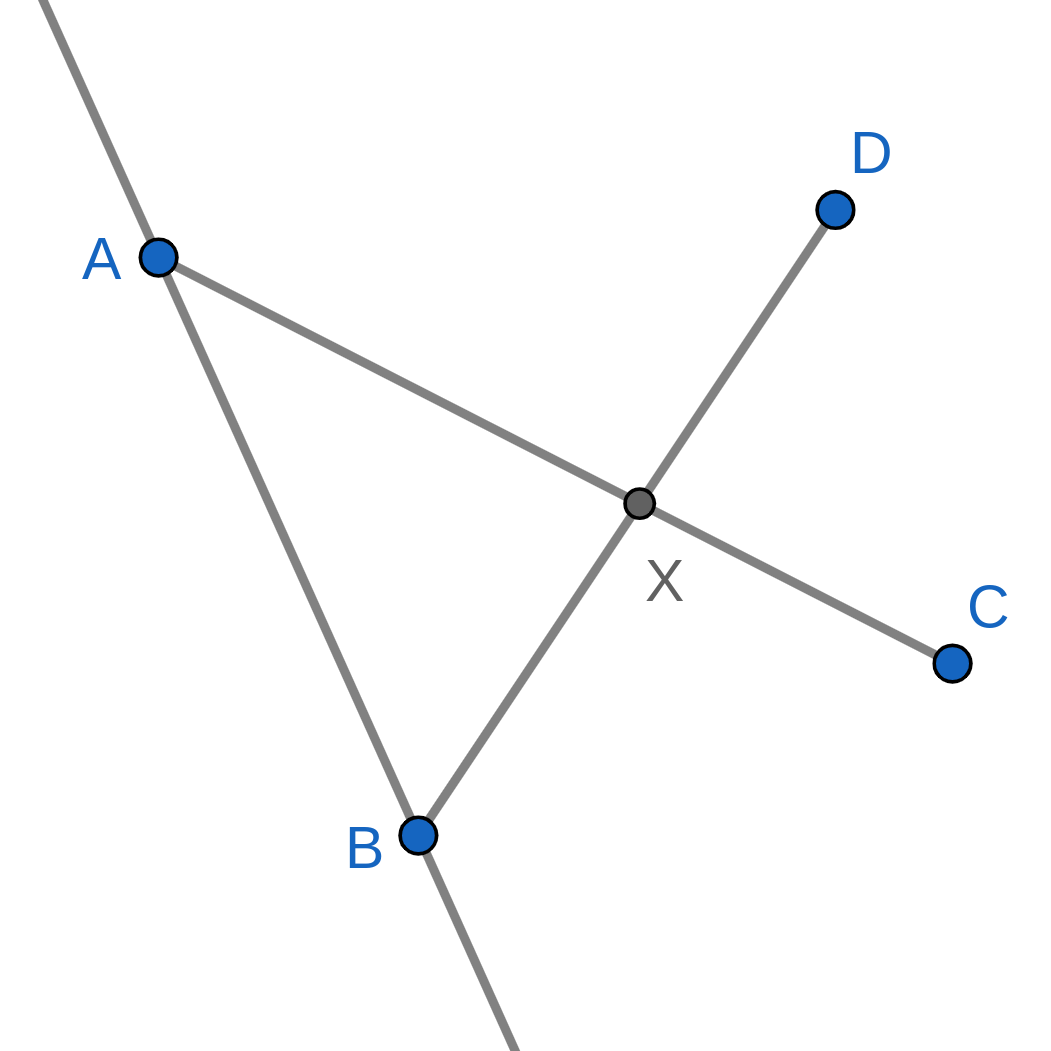
\includegraphics{images/convex_3.png}
\end{marginfigure}


Since our quadrilateral is convex, the diagonal segments $AC$ and $BD$ meet at a point $X$. By Lemma \ref{lemma:same-side-ray}, $C$ and $X$ lie on the same side of $AB$, and also $X$ and $D$ lie on the same side of $AB$. By Lemma \ref{lemma:same-side-transitive}, $C$ and $D$ lie on the same side of line $AB$. Since our original pair of adjacent vertices is chosen arbitrarily, this holds for all such pairs. This means that (2) is true.

\item[(3) implies (1):] Suppose that we have a quadrilateral $ABCD$ which satisfies condition (2). We must show that the diagonal segments $AC$ and $BD$ meet.

Consider the angle $ABC$. By Lemma \ref{lemma:lighthouse}, the ray $BD$ meets the segment $AC$ at a point $X$. We want to show that $X$ lies between $B$ and $D$.

\begin{marginfigure}
  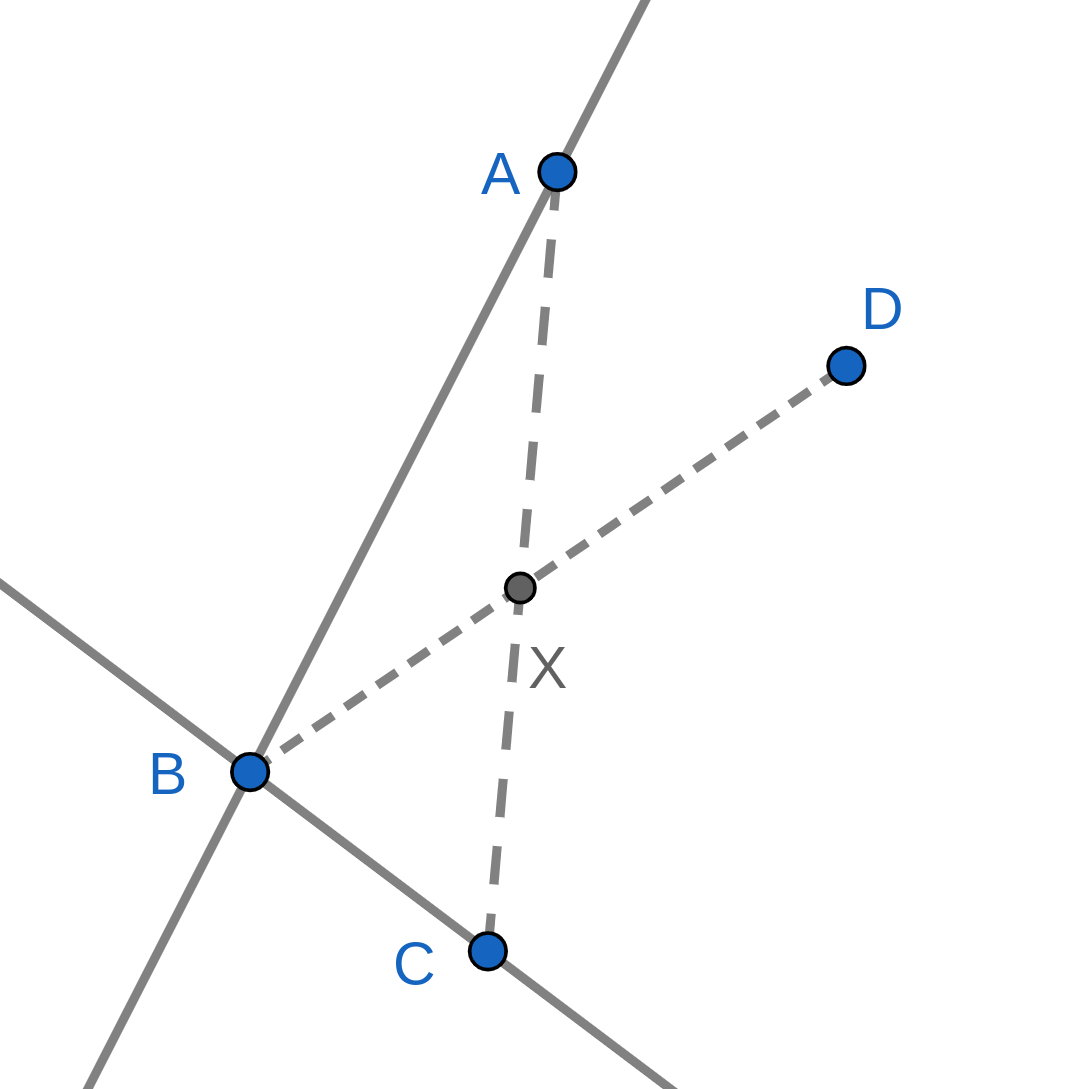
\includegraphics{images/convex_4.png}
\end{marginfigure}

Suppose instead that $D$ lies between $B$ and $X$. Then $D$ lies inside the triangle $ABC$. By Lemma \ref{lemma:lighthouse}, the ray $CD$ crosses through the segment $AB$. This means that $A$ and $B$ lie on opposite sides of line $CD$, and hence $A$ Does not lie inside angle $BCD$. That contradicts condition (3), as $B$, $C$, and $D$ are consecutive vertices.


\begin{marginfigure}
  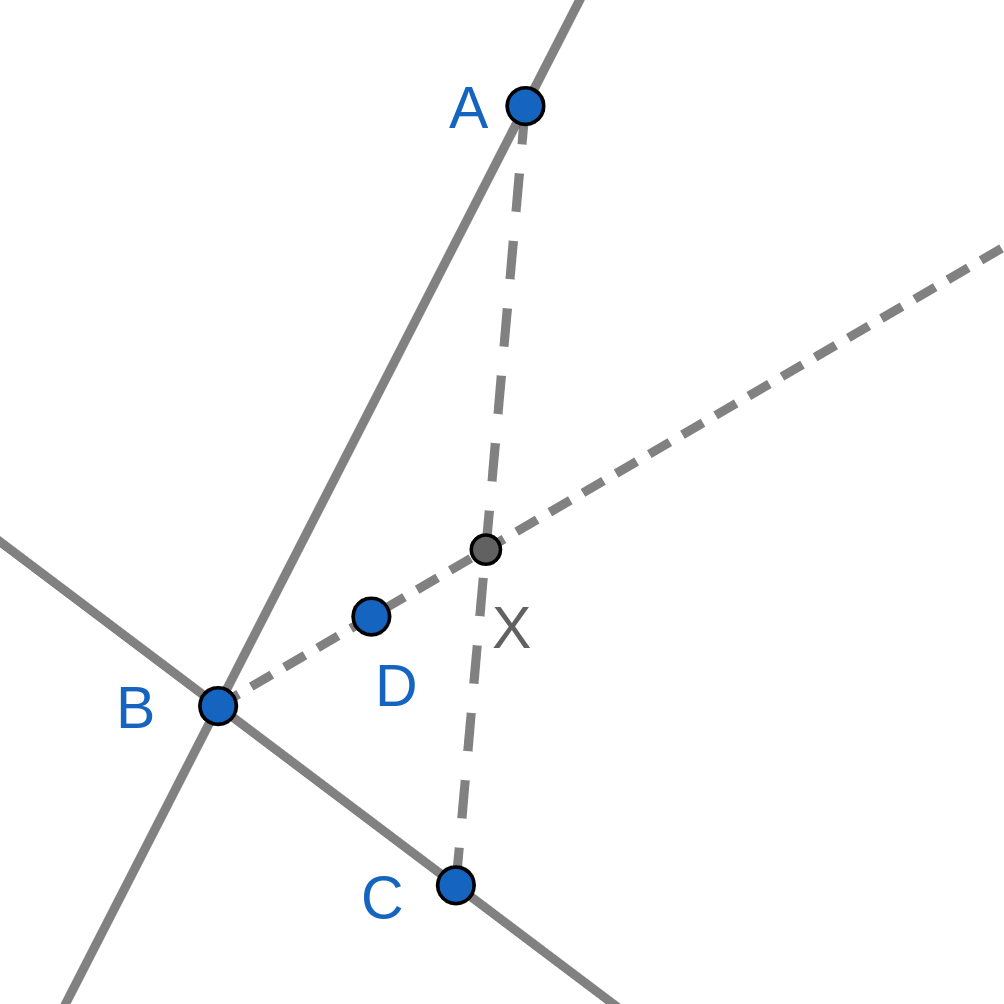
\includegraphics{images/convex_5.png}
\end{marginfigure}


We conclude that $X$ lies between $B$ and $D$, so the segments $AC$ and $BD$ meet, and $ABCD$ is convex.
\end{description}
\end{proof}

\clearpage

%%%%%%%%%%%%%%%%%%%%%%%%%%%%%%%%%%%%%%%%%%%%%%%%%%%%%%
\setcounter{section}{3}
\setcounter{theorem}{0}
\section{The Rectangle, and Parallelism}\label{section:rectangles}

\begin{theorem}[Conjecture 3.1]\label{theorem:rectangle-parallelogram}
If $ABCD$ is a rectangle, then $ABCD$ is a parallelogram.
\end{theorem}

\begin{proof}
We must show that each pair of opposite sides of $ABCD$ extends to a pair of parallel lines. To this end, extend sides $AB$, $CD$, and $BC$ to lines.  Choose a point $X$ on line $AB$ so that $B$ lies between $A$ and $X$. Choose a point $Y$ on line $BC$ so that $B$ lies between $Y$ and $C$.

By Euclid's Proposition I.15, angle $YBX$ is congruent to angle $ABC$. Therefore $YBX$ is a right angle. Note that line $AB$ falls upon the lines $AD$ and $BC$. Since $BAD$ is also a right angle, we have that the exterior angle $YBX$ is congruent to the interior angle opposite side, namely $BAD$. So by Euclid's Proposition I.29, the lines $AC$ and $BD$ are parallel.

In the same manner, we argue that the lines $AB$ and $CD$ are parallel, as they are fallen on by $BC$ in a way that makes all right angles at each intersection.
\end{proof}


\begin{theorem}[Conjecture 3.2]\label{theorem:rectangle-opp-sides}
Let $ABCD$ is a rectangle, then $AB$ is congruent to $CD$ and $AD$ is congruent to $BC$.
\end{theorem}

\begin{proof}
By Theorem \ref{theorem:rectangle-parallelogram}, $ABCD$ is also a parallelogram. By Euclid's Proposition I.34, both pairs of its opposite sides are congruent.
\end{proof}


\begin{theorem}[Conjecture 3.3]
Let $ABCD$ be a rectangle. The diagonal segments $AC$ and $BD$ meet.
\end{theorem}

\begin{proof}
Note that the angle $ABD$ is less than the angle $ABC$, being only a part of it. Similarly, the angle $BAC$ is less than angle $BAD$. Also, angles $ABC$ and $BAD$ taken together make two right angles. Therefore, angles $ABD$ and $BAC$ taken together make less than two right angles. Since these angles make less than two right angles, by Postulate 5 we deduce that the rays $AC$ and $BD$ meet.

By changing the letters around in the argument, we may work on the opposite side of the rectangle. From this, we deduce that the rays $CA$ and $DB$ meet.

Since the lines $AC$ and $BD$ can meet only once, these two intersections must be the same point. Therefore, this point of intersection must be on the segments $AC$ and $BD$.
\end{proof}

\clearpage

\begin{theorem}[Conjecture 3.3]
\label{theorem:rectangle-diags-cong}
Let $ABCD$ be a rectangle. The diagonal segments $AC$ and $BD$ are congruent.
\end{theorem}

\begin{proof}
By Theorem \ref{theorem:rectangle-opp-sides}, we know that segment $BC$ is congruent to segment $AD$. The angles $CBA$ and $DAB$ are both right angles, and therefore congruent. Of course, the segment $AB$ is congruent to itself. Therefore, by Euclid's Proposition I.4, triangle $ABC$ is congruent to triangle $BAD$. Since the segments $AC$ and $BD$ are corresponding parts of these triangles, they must be congruent, by the definition of congruent triangles.
\end{proof}


\begin{theorem}[Conjecture 3.3]
Let $ABCD$ be a rectangle. Let $X$ be the point where $AC$ and $BD$ meet. Then $X$ is the midpoint of both segments.
\end{theorem}

\begin{proof}
By Theorem \ref{theorem:rectangle-parallelogram}, the rectangle $ABCD$ is a parallelogram. Note that the diagonal line $AC$ falls upon the parallel lines $AD$ and $BC$. Therefore, by Euclid's Proposition I.29, the angles $BCA$ and $DAC$ are congruent. Similarly, the diagonal $BD$ falls on the parallel lines $AD$ and $BC$. Again by Proposition I.29, the angles $CBD$ and $BDA$ are congruent. 

By Theorem \ref{theorem:rectangle-opp-sides}, the segment $BD$ is congruent to the segment $AD$. Therefore, by Euclid's Proposition I.26, triangle $XDA$ is congruent to triangle $XBC$.

By the definition of congruent triangles, the corresponding segments are congruent, namely $AX$ is congruent to $CX$ and $BX$ is congruent to $DX$. By the definition of a midpoint, this means that $X$ is the midpoing of both segment $AC$ and segment $BD$.

\end{proof}





\begin{theorem}[Conjectures 3.4, 3.8, \& 3.9]
There exists a quadrilateral $ABCD$ for which the following are true:
\begin{itemize}
\item angle $ABC$ and angle $ADC$ are right angles,
\item side $AB$ is congruent to $CD$,
\item side $BC$ is congruent to side $AD$,
\item side $BC$ meets side $AD$,
\item angles $BCD$ and $DAB$ are congruent, and each is less than a right angle.
\end{itemize}
In particular, this quadrilateral $ABCD$ is not a rectangle.
\end{theorem}

\begin{theorem}[Conjecture 3.4]
add convexity or simplicity
\end{theorem}


\begin{definition}
A quadrilateral is called \emph{simple} if for each pair of its sides, those sides can only meet at a common vertex of the quadrilateral.
\end{definition}

\begin{theorem}[Conjecture 3.5]
Let $ABCD$ be a quadrilateral such that the angles $ABC$ and $ADC$ are right angles, and lines $AB$ and $DC$ are parallel. Then $ABCD$ is a rectangle.
\end{theorem}

\begin{theorem}[Conjecture 3.6: The Midline Theorem]
Let $ABC$ be a triangle. Let $D$ be the midpoint of $AB$ and $E$ the midpoint of $AC$. The line $DE$ is parallel to the line $AB$.
\end{theorem}

\begin{theorem}[Conjecture 3.7: Varignon's Theorem]
Let $ABCD$ be a quadrilateral. Let $W$, $X$, $Y$, and $Z$ be the midpoints of $AB$, $BC$, $CD$, and $DA$, respectively. When the four points $W$, $X$, $Y$, and $Z$\marginnote{Sometimes these four points end up collinear.} form a quadrilateral, then this quadrilateral is a parallelogram.
\end{theorem}

\begin{theorem}[Conjecture 3.8]
add convexity or simplicity?
\end{theorem}


\begin{theorem}[Conjecture 3.9]
add convexity or simplicity?
\end{theorem}


\clearpage
%%%%%%%%%%%%%%%%%%%%%%%%%%%%%%%%%%%%%%%%%%%%%%%%%
\setcounter{section}{4}
\setcounter{theorem}{0}
\section{Skepticism}\label{section:skepticism}




\end{document}


